% TODO add tech / software table?
\section{Materials and methods}

\subsection{Study design}

The study had two main goals.
Firstly, I aimed to develop a map interface for
interactively presenting an extensive spatial dataset on travel times,
and through the development process assess
the tools and options available for making such a map.
More precisely,
I focused on the choice of web mapping library
and on the different approaches in preprocessing the mapped data.
The goal was to find how,
and to what extent,
these factors affect the map interface.
The second goal was to understand how map users utilize such a map interface,
and how the interactive map works as a representation.
Here I employed a survey to find out how
people use the map when given different tasks to complete with it,
and whether a highly interactive presentation approach affects
how map users perceive the mapped phenomenon and interpret the map.
These two themes, the development process and the survey,
make up the two high-level components of the study.

% While the primary goal of the development process was
% to produce the map presentation and enable the survey,
% the development process in and of itself was crucial to the study as well.
% Its purpose was to be the framework that
% allows for answering the research questions
% about the more technology-centric aspects of
% the making of an interactive map.

Pragmatically speaking, a large part of this study was
a software development project to produce a functional web map application,
and the parts that were not, were still reliant on
the software development project succeeding.
This naturally affected the study design.
It allowed for freedom in crafting a map interface made exactly for this study,
but also introduced limitations
as any functionality to be included in the map, and in the study,
had to also be implemented.
In other words, the technical implementation as well as the survey
had to be designed around what is meaningful to study,
but also based on what is realistic to implement.
To minimize the risk and uncertainty inherent to such a setting,
I heavily utilized modern software development methodologies
\parencite{saq2020, bec2001, sha2017, kuh2017}
in planning the development process and the study as a whole.
Based on these,
I formatted the following points of focus
to guide the development process:
\begin{itemize}
	\item Plan minimally and adapt the plan constantly.
	\item Prioritize a working state of the entire application over details in single components.
	\item Adapt to technical constraints at the start, not at the end.
\end{itemize}

By adhering to these principles I could at an early stage see
whether the study was realistic, and,
especially considering the more technology-centric side of the study,
hone in on what research questions were actually meaningful.
Iteratively improving the application as a functional whole
allowed me to consider the map interface
from the perspective of the map user as early as possible,
better integrating the survey into the study.
This is important as the map presentation is simultaneously an output of the development process
and an input to the design of the survey.

For an overview of the study design see figure \ref{fig:study design}.
% This allowed me to improve the relevancy of my research. TODO Discussion?
% I say this not only in the context of gaining valuable results to my research questions --
% I want to emphasize that to even know what research questions to ask is impossible with a linear approach.

% While the development process and the survey were linked to each other,
% they each had their separate goals and outputs too.
% In addition to producing the map presentation,
% the development process had to enable testing and answering my research questions
% about the making of an interactive map.
% This placed increased
% The goal of the survey is to gain insight on
% how the interactive map works as a representation of the mapped phenomenon.
% With the survey I collect data on map usage,
% which I in turn analyse to answer my research questions related to the map usage.

\begin{figure}[H]
	\centering
	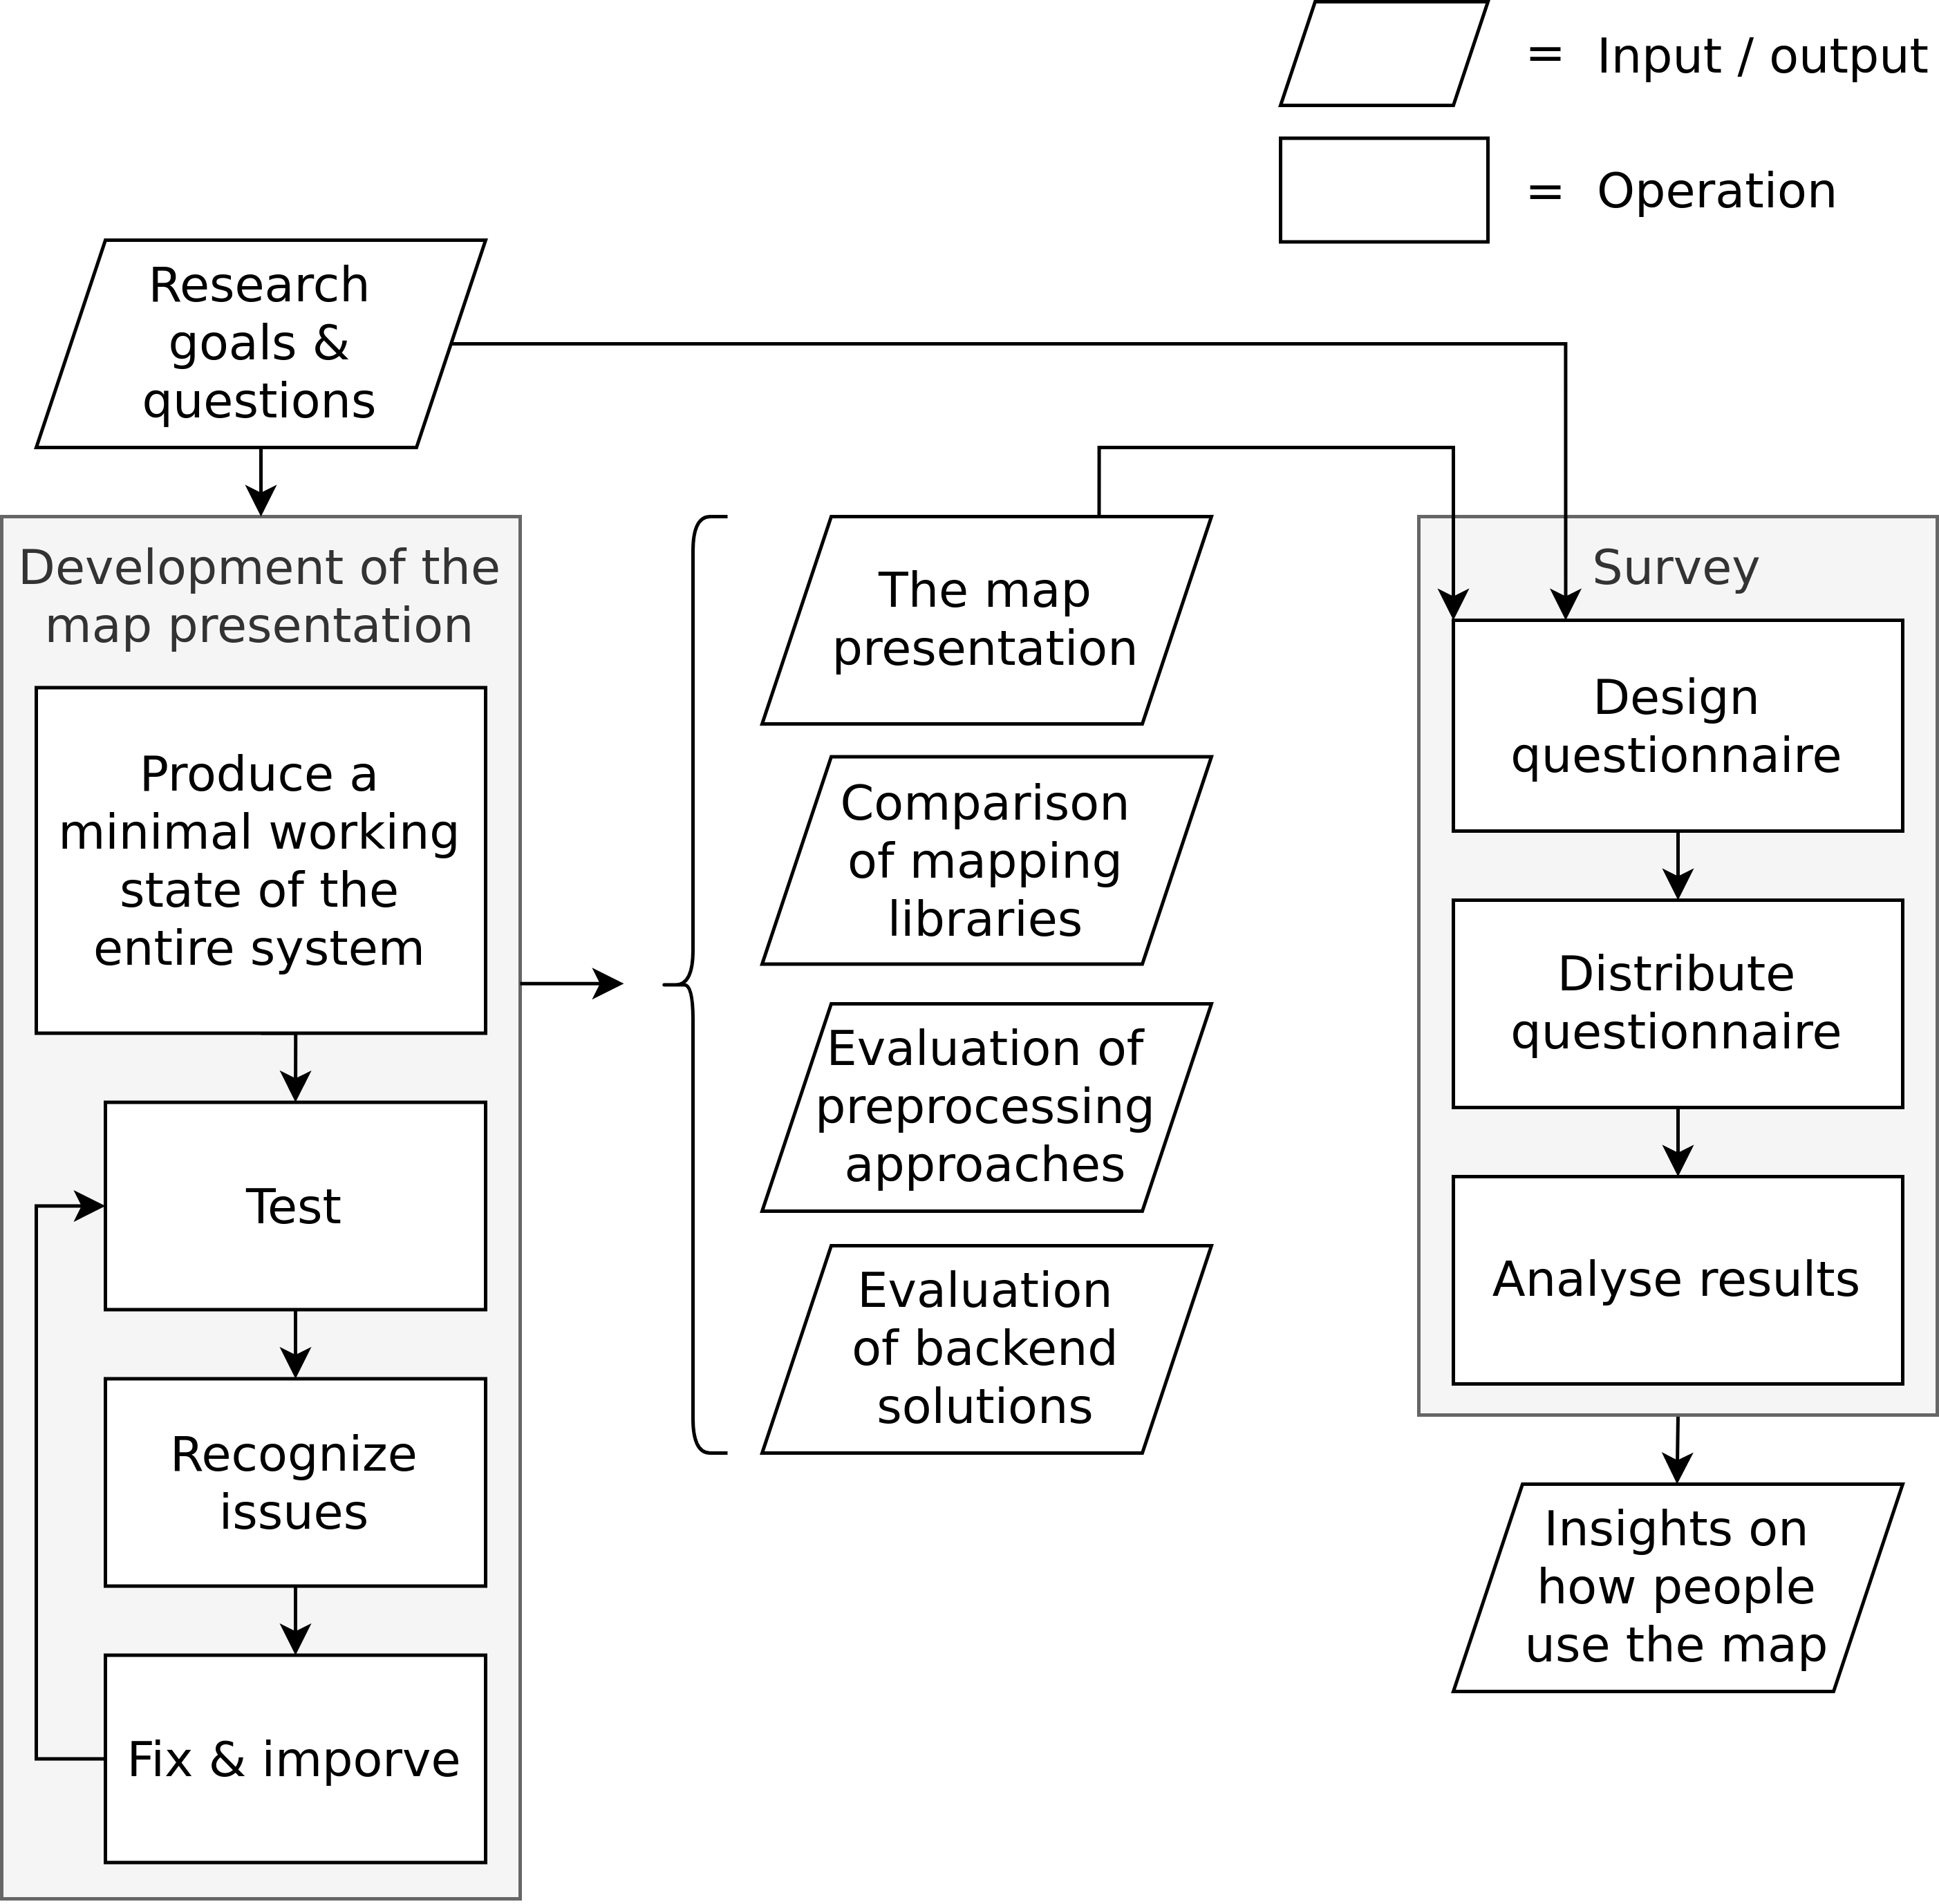
\includegraphics[width=\diagramwidth]{visual/figures/diagrams/study_design.png}
	\caption{An overview of the study design.}
	\label{fig:study design}
\end{figure}


\subsection{Data -- Helsinki region Travel Time Matrix}

The \acrlong{ttm} (\acrshort{ttm}) \parencite{fin2023}
is a dataset containing information of travel times and distances
in the Helsinki region in southern Finland.
This dataset was crucial to developing the map application,
as it was the sole source of the travel times shown on the map.
The dataset and the set of methods with which it is produced are open-source.

% Describe ttm in general: ykr, origin dest pairs etc (more surface level stuff common to all matrices)
A significant component of the \acrshort{ttm} is the \acrlong{ykr} (\acrshort{ykr})
statistical grid made by the Finnish Environmental Institute.
The grid has a spatial resolution of 250x250m, and it covers the entire Finland.
Most importantly, however, the part of the \acrshort{ykr} grid that overlaps with
the Helsinki region provides the spatial component for
the travel times stored in the \acrshort{ttm}.
The spatial extent of the dataset is shown in figure \ref{fig:ttm extent}.

\begin{figure}[H]
	\centering
	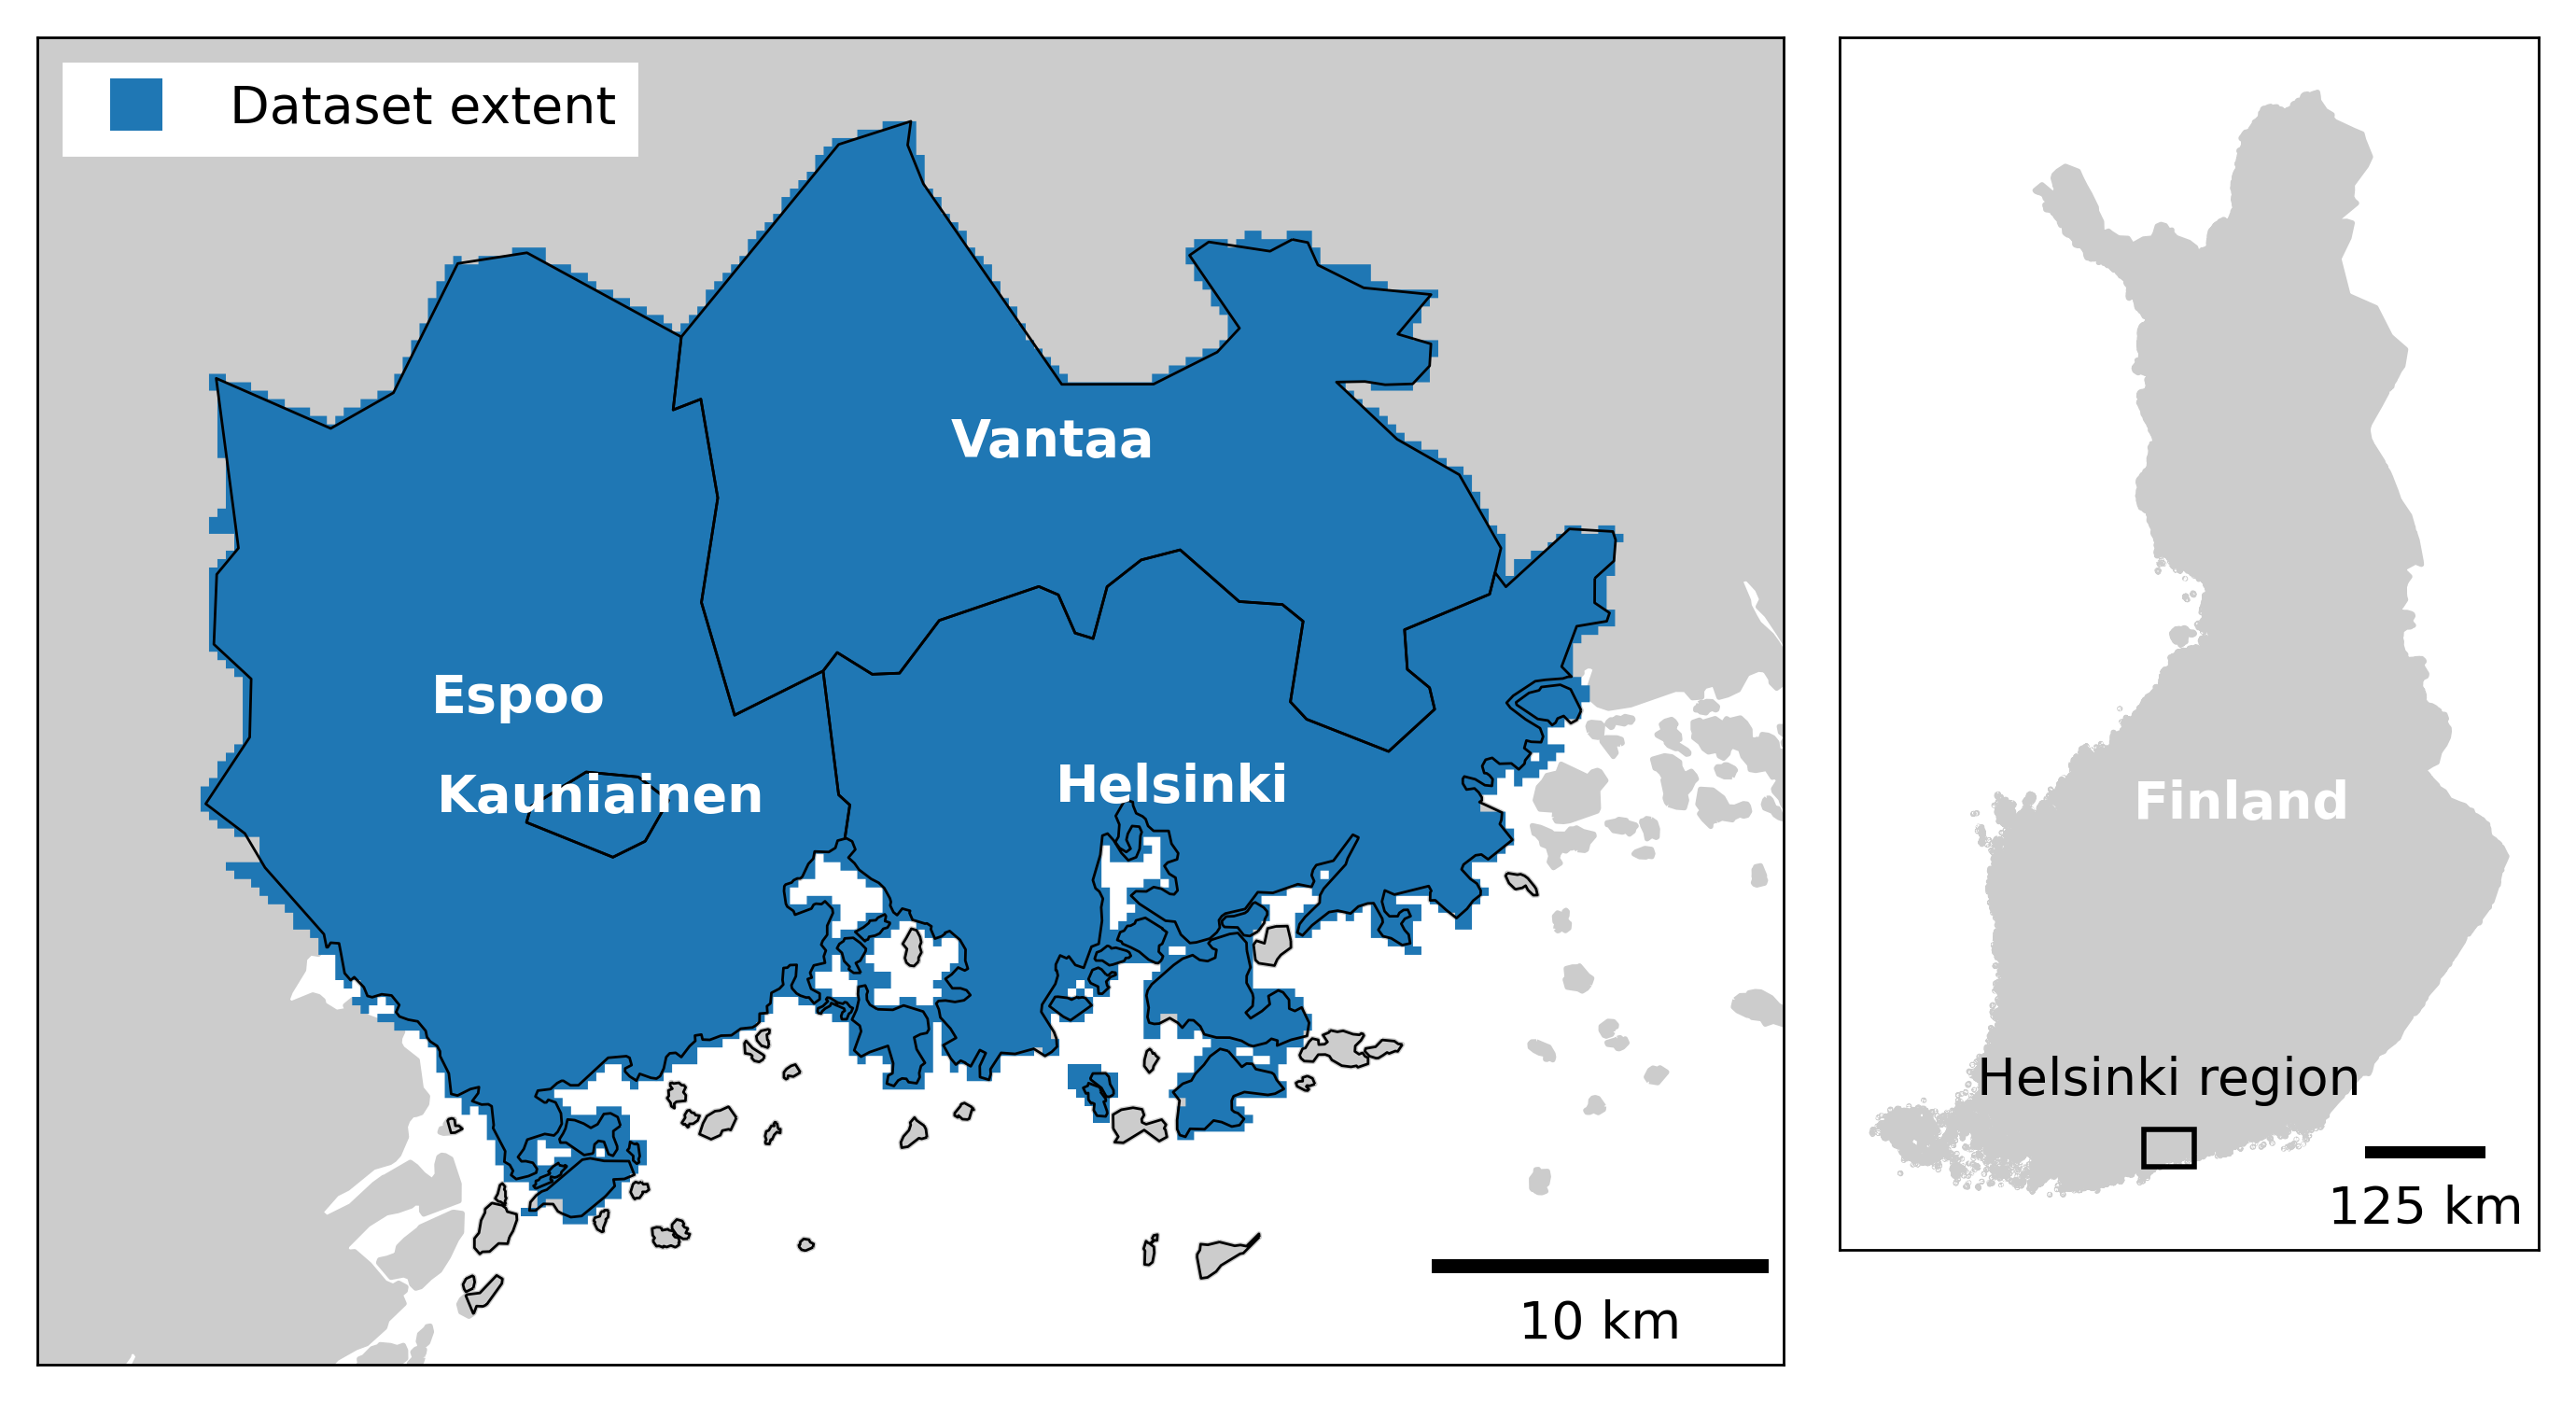
\includegraphics[width=0.9\textwidth]{visual/figures/ttm/ttm_extent}
	\caption{The location and extent of the TTM}
	\label{fig:ttm extent}
\end{figure}

The \acrshort{ttm} stores the travel times and distances
from every \acrshort{ykr} grid cell to every other  \acrshort{ykr} grid cell
within the Helsinki region.
The Helsinki region fits 13231 \acrshort{ykr} grid cells,
which means that the complete \acrshort{ttm} contains travel times and distances for
over 175 million routes.

All the routes are calculated for multiple different travel modes.
The primary travel modes are walking, cycling, public transportation and private car,
and, when applicable, each mode has variations based on
time of day and / or walking or cycling speed.
The time of day is especially relevant to motorized transport
in the form of the rush hour, for example,
while walking speed affects any travel mode
where a significant portion of the trip is covered on foot.
To be comparable with each other,
the travel times for all travel modes are
calculated with a \textit{door-to-door approach}
which accounts for things such as walking to a bus stop,
waiting for transfer times based on public transit schedules,
or locking and unlocking a bike \parencite{ten2020}.

% Describe the particular matrix (2023), methodology etc
\acrshort{ttm}s have been calculated for multiple years.
Differences between these datasets exist in the applied methodologies
and, thus, also in the content \parencite{ten2020}.
Also, the underlying city structure as well as the street and public transport networks
are by no means static over the years
which further introduces differences.
The map presentation I developed in this study
is based on the 2023 version of the \acrshort{ttm},
the newest one at the time of writing.
See table \ref{tab:ttm description} for an overview of the dataset,
and table \ref{tab:ttm table structure} for all the travel modes and
their variations included in the dataset.

\begin{table}[H]
	\caption{Descriptive values of the \acrshort{ttm}}
	\label{tab:ttm description}
	\centering
	\begin{tabular}{ | L{0.4\textwidth} | L{0.5\textwidth} | }
		\hline
		Spatial resolution
		& 250 x 250 m
		\\
		\hline
		Number of grid cells
		& 13231
		\\
		\hline
		Number of origin-destination pairs
		& 175 059 361
		\\
		\hline
		Travel modes
		& \tabitem walking \\
		& \tabitem cycling \\
		& \tabitem public transportation \\
		& \tabitem private car \\
		\hline
		Travel mode variations (if applicable)
		& \tabitem Time of day (rush hour, midday, night) \\
		& \tabitem Walking speed (average, slow) \\
		& \tabitem Cycling speed (average, fast, slow) \\
		\hline
	\end{tabular}
\end{table}


\begin{table}[H]
	\caption{The table structure of \acrshort{ttm} data}
	\label{tab:ttm table structure}
	\centering
	\begin{tabular}{ | L{0.15\textwidth} | L{0.75\textwidth} | }
		\hline
		\textbf{Column name}
		& \textbf{Description}
		\\
		\hline
		\hline
		from\_id
		& ID number of the origin grid cell
		\\
		\hline
		to\_id
		& ID number of the destination grid cell
		\\
		\hline
		walk\_avg
		& Travel time in minutes from origin to destination by walking at an average speed
		\\
		\hline
		walk\_slo
		& Travel time in minutes from origin to destination by walking slowly
		\\
		\hline
		bike\_avg
		& Travel time in minutes from origin to destination by cycling at an average speed; incl. extra time (1 min) to unlock and lock bicycle
		\\
		\hline
		bike\_fst
		& Travel time in minutes from origin to destination by cycling fast; incl. extra time (1 min) to unlock and lock bicycle
		\\
		\hline
		bike\_slo
		& Travel time in minutes from origin to destination by cycling slowly; incl. extra time (1 min) to unlock and lock bicycle
		\\
		\hline
		pt\_r\_avg
		& Travel time in minutes from origin to destination by public transportation in rush hour traffic, walking at an average speed
		\\
		\hline
		pt\_r\_slo
		& Travel time in minutes from origin to destination by public transportation in rush hour traffic, walking at a slower speed
		\\
		\hline
		pt\_m\_avg
		& Travel time in minutes from origin to destination by public transportation in midday traffic, walking at an average speed
		\\
		\hline
		pt\_m\_slo
		& Travel time in minutes from origin to destination by public transportation in midday traffic, walking at a slower speed
		\\
		\hline
		pt\_n\_avg
		& Travel time in minutes from origin to destination by public transportation in nighttime traffic, walking at an average speed
		\\
		\hline
		pt\_n\_slo
		& Travel time in minutes from origin to destination by public transportation in nighttime traffic, walking at a lower speed
		\\
		\hline
		car\_r
		& Travel time in minutes from origin to destination by private car in rush hour traffic
		\\
		\hline
		car\_m
		& Travel time in minutes from origin to destination by private car in midday traffic
		\\
		\hline
		car\_n
		& Travel time in minutes from origin to destination by private car in nighttime traffic
		\\
		\hline
		walk\_d
		& Distance from origin to destination, in metres, on foot
		\\
		\hline
	\end{tabular}
\end{table}




\subsection{Implementation of the map presentation}

\subsubsection{Software requirements}
% The requirements of the application are an essential aspect to consider,
% since they
% For example, the sheer scale and detail of the dataset being visualized
% means that instantaneous interaction with the map is not realistic
% if no detail of the mapped data is to be sacrificed.
% These kinds of tradeoffs are important to recognize,
% because only through them is it possible to specify what
% requirements should, or even could, be placed on the map application.

% TODO copypasta

% Roughly what kind of a map? Why?
% Based on the background study,  % TODO
Software requirements are the functionalities and properties
that a given system should have,
as well as the constraints it must adhere to \parencite{chu2009}.
They are an essential aspect to consider in software development
as they are a way to explicate
what is being developed and what exactly is the framework
in which an implementation process is carried out \parencite{saq2020}.
Software requirements are often divided into
functional and nonfunctional requirements.
Functional requirements define the user-facing features of the system
while nonfunctional requirements describe the properties of a system
\parencite{chu2009}.
Nonfunctional requirements can be further divided into
quality attributes and constraints.
Quality attributes describe \textit{how} the software should be,
while constraints most often refer to technical limitations \parencite{chu2009}.

The starting point for specifying the requirements of the map application
was the decision to prioritize real-time interaction over minute detail in the map interface.
The goal of the map interface was to act as a dynamic overview to the entire \acrshort{ttm}.
As mentioned in the previous section,
the spatial dimension of the \acrshort{ttm} is large.
If all of it is to be explored,
an interaction exchange to select and re-select different locations to map
should be as effortless and instantaneous as possible.
The other dimension, travel mode, is much smaller,
but should also be interactively selectable.
These two goals, while still quite vague,
immediately placed a number of requirements on the application.
From the perspective of the user,
there must be functionalities for interacting with the map to
select different locations, preferably very rapidly,
and for selecting different travel modes.
A significant quality attribute to consider is that the application should
be responsive enough for instantaneous real-time interactivity.

From a technology-centric perspective an essential factor was
the decision to target the web as the platform.
This constraint was the starting point for considering the technologies
of the implementation.
From an architectural standpoint,
it meant that the application is more specifically a \textit{web application}
consisting of a frontend (a map interface) and a backend
(a solution for getting data to the map interface running on the client).
So, in further references to an \textit{application},
I mean the functional whole made of a map interface (frontend) and data access (backend)
\parenfig{web map app}.

\begin{figure}[H]
	\centering
	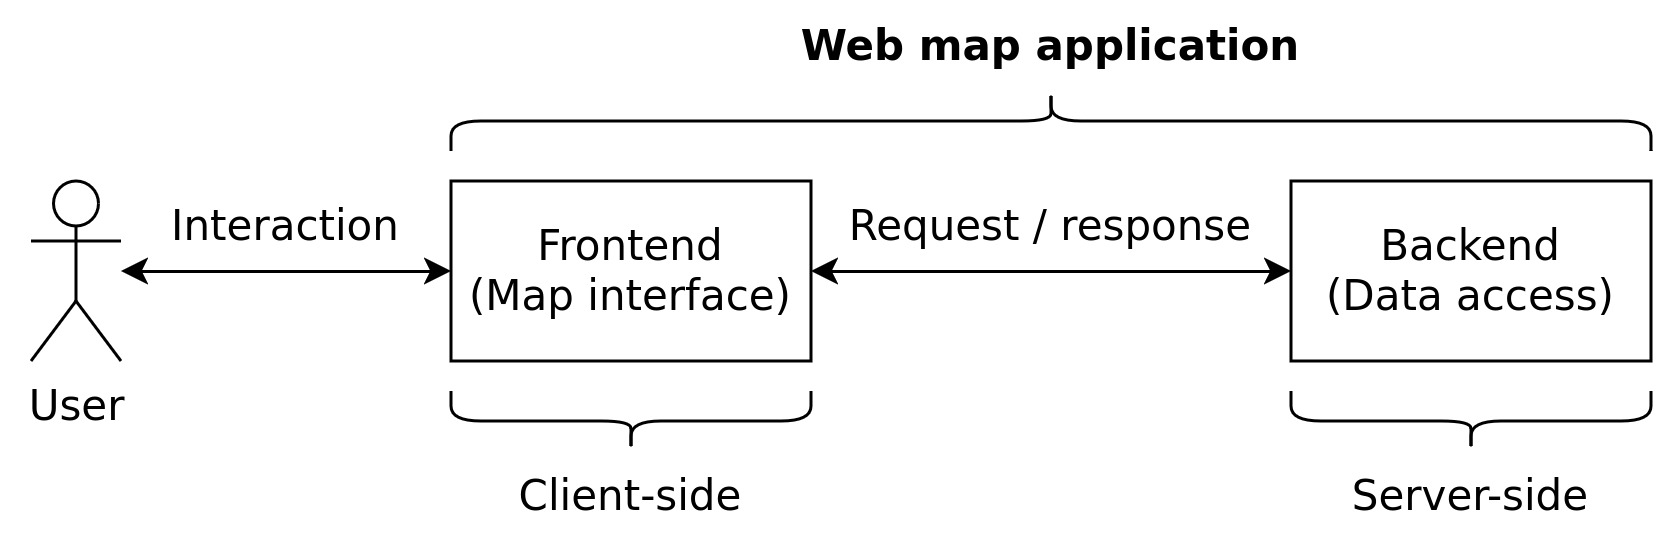
\includegraphics[width=\diagramwidth]{visual/figures/diagrams/web_map_app}
	\caption{
		A web map application like the one described above requires
		a frontend for providing the map interface
		and a backend for supplying the frontend with data to map.
	}
	\label{fig:web map app}
\end{figure}

I specified the software requirements at this quite non-detailed
level at first.
In accordance with the guideline of continuous adaptation,
\parencite{bec2001} I further focused them only as the application
and the study took shape.
However, to communicate the development and study process in an orderly manner,
and to motivate the design decisions I've made,
I present the requirements of the final application here.
Still, I should emphasize that the reality is not this linear.

The functional requirements specify the styles and modes of interaction,
as well as the set of operations a user can carry out with the map.
Firstly, the map should have two modes of interaction for selecting locations to be mapped.
These include clicking the map with a pointing device to produce a map of the clicked location,
and continuously changing the mapped location by moving the cursor over the map
(referred to as hovering).
This enables comparing two different levels of interactivity in the study:
clicking to produce static maps and hovering to produce
a responsive, \enquote{live},
representation of the accessibility under the cursor.
There should also be interface capabilities for selecting travel modes
and changing the mode of location selection.
To facilitate the exploration of the mapped area
at different points of focus and levels of detail,
the map should support panning and zooming the view.
The functional requirements are documented in table \ref{tab:functional requirements}.

For the quality attributes of the application,
performance is an essential consideration --
both in the sense of software performance
and the responsiveness of the application as perceived by the user.
This must be considered in both the front and backend of the application.
Quality attributes that are invisible to a user, but still vital,
are that the application can be maintained and deployed,
and that it can meet different real-world usage loads.
If these attributes were lacking,
the application would have little real value.
The \textit{deployment environment},
in other words the computing platform onto which the server-side of the application is deployed,
is the container orchestration platform \textit{Rahti} provided by the \presentacr{csc}.
Rahti is based on the \textit{OpenShift} platform,
which in turn runs on \textit{Kubernetes}.
Kubernetes is a container orchestration tool
that allows for declaratively managing clusters
of containerized applications and their accompanying services.
I mention these details because to the application they are constraints:
Both the front and backend implementations should be completely containerized,
and they both are deployed with the OpenShift flavour of Kubernetes.
Also, as is obvious by now,
the frontend of the application is constrained to running in a web browser.
For the nonfunctional requirements of the application,
see table \ref{tab:nonfunctional requirements}.

\begin{table}[H]
	\caption{The functional requirements of the map application}
	\label{tab:functional requirements}
	\centering
	\begin{tabular}{ | L{0.3\textwidth} | L{0.6\textwidth} | }
		\hline
		Requirement
		& Description
		\\
		\hline
		\hline
		Location selection by clicking
		& The user can click on a location and produce an accessibility map of that location.
		\\
		\hline
		Location selection by hovering
		& The user can hover their mouse over the map,
		and the map shows the accessibility of the location that is under the cursor,
		updating constantly as the cursor moves.
		\\
		\hline
		Toggling between modes of location selection
		& The user can toggle their mode of interaction by clicking:
		Clicking while hovering locks the map, clicking while the map is locked resumes hovering.
		\\
		\hline
		Interactive selection of travel mode
		& The user can choose the travel mode for which the travel times shown on the map are calculated.
		\\
		\hline
	\end{tabular}
\end{table}

\begin{table}[H]
	\caption{
		The nonfunctional requirements of the map application specify
		its desired qualities (\ref{tab:quality attributes}) and
		the constraints it must adhere to (\ref{tab:constraints}).
	}
	\label{tab:nonfunctional requirements}
	\begin{subtable}[h]{\textwidth}
		\caption{}
		\label{tab:quality attributes}
		\centering
		\begin{tabular}{ | L{0.2\textwidth} | L{0.7\textwidth} | }
			\hline
			\textbf{Category}
			& \textbf{Requirements}
			\\
			\hline
			\hline
			Performance
			& \tabitem Data serving speed allows for real-time interaction. \\
			& \tabitem Map rendering speed allows for real-time interaction. \\
			\hline
			Maintainability
			& \tabitem All components are as independent as possible. \\
			& \tabitem The codebase is versioned and documented. \\
			& \tabitem Deploying the application is reproducible. \\
			\hline
			Usability
			& \tabitem Visual feedback from user interaction is instantaneous. \\
			\hline
			Scalability
			& \tabitem The application is scalable to meet different usage loads. \\
			& \tabitem Different application components can be scaled independently. \\
			\hline
		\end{tabular}
	\end{subtable}
	\newline
	\newline  % https://tex.stackexchange.com/questions/38893/cant-generate-vertical-space-between-tables
	\newline
	\begin{subtable}[h]{\textwidth}
		\caption{}
		\label{tab:constraints}
		\centering
		\begin{tabular}{ | L{0.2\textwidth} | L{0.7\textwidth} | }
			\hline
			\textbf{Type of constraint}
			& \textbf{Description}
			\\
			\hline
			\hline
			Client-side platform
			& The frontend of the map application runs in a web browser.
			\\
			\hline
			Deployment environment
			& The front and backend are deployed in containers
			utilizing the OpenShift container platform.
			\\
			\hline
		\end{tabular}
	\end{subtable}
\end{table}


\subsubsection{Assessing data preprocessing approaches}
% The need for preprocessing
% - what would raw data be like?
% - why as much as possible should be precalculated
% && the requirements preprocessing must satisfy
Preprocessing and simplifying the \acrshort{ttm} was a significant part of the study.
With initial testing,
it became obvious that
using unprocessed \acrshort{ttm} data,
i.e. the complete 13000-cell grid of travel times for every location,
was not an option due to two issues:
unresponsiveness of the map interface and the large file sizes.
Based on this,
I formed the hypothesis that either the file sizes
or the geometrical complexity of the data would be
the major factor limiting the responsiveness of the map,
i.e. the performance bottleneck.

So it was clear that
some type of preprocessing as well as simplification of the 
\acrshort{ttm} data was necessary --
both to test the hypothesis and to enable real-time interaction in the map.
The goal of assessing different approaches to data preprocessing, thus,
was to find the suitable level and types of simplification,
and to compare the effectiveness of different approaches.

When assessing the preprocessing approaches, I focused on:
\begin{itemize}
	\item The impact on file size, and thus on the speed of transferring data over internet.
	\item The impact on rendering speed of the map when mapping the data.
	\item The impact on the amount of information on the map,
	i.e. how much visual information is lost when a given approach is applied.
\end{itemize}

I assessed four types of preprocessing approaches:
\begin{itemize}
	\item Aggregation of travel time data into isochrone polygons \parenfig{isochrone intervals}
	\item Limiting the maximum travel time, i.e. the geographical extent of the results \parenfig{tt limits}
	\item Reducing the coordinate precision of geometries
	\item Minimizing files (simplifying GeoJSON structure, compression using gzip)
\end{itemize}

\begin{figure}[H]
	\centering
	\begin{subfigure}[b]{0.5\textwidth}
		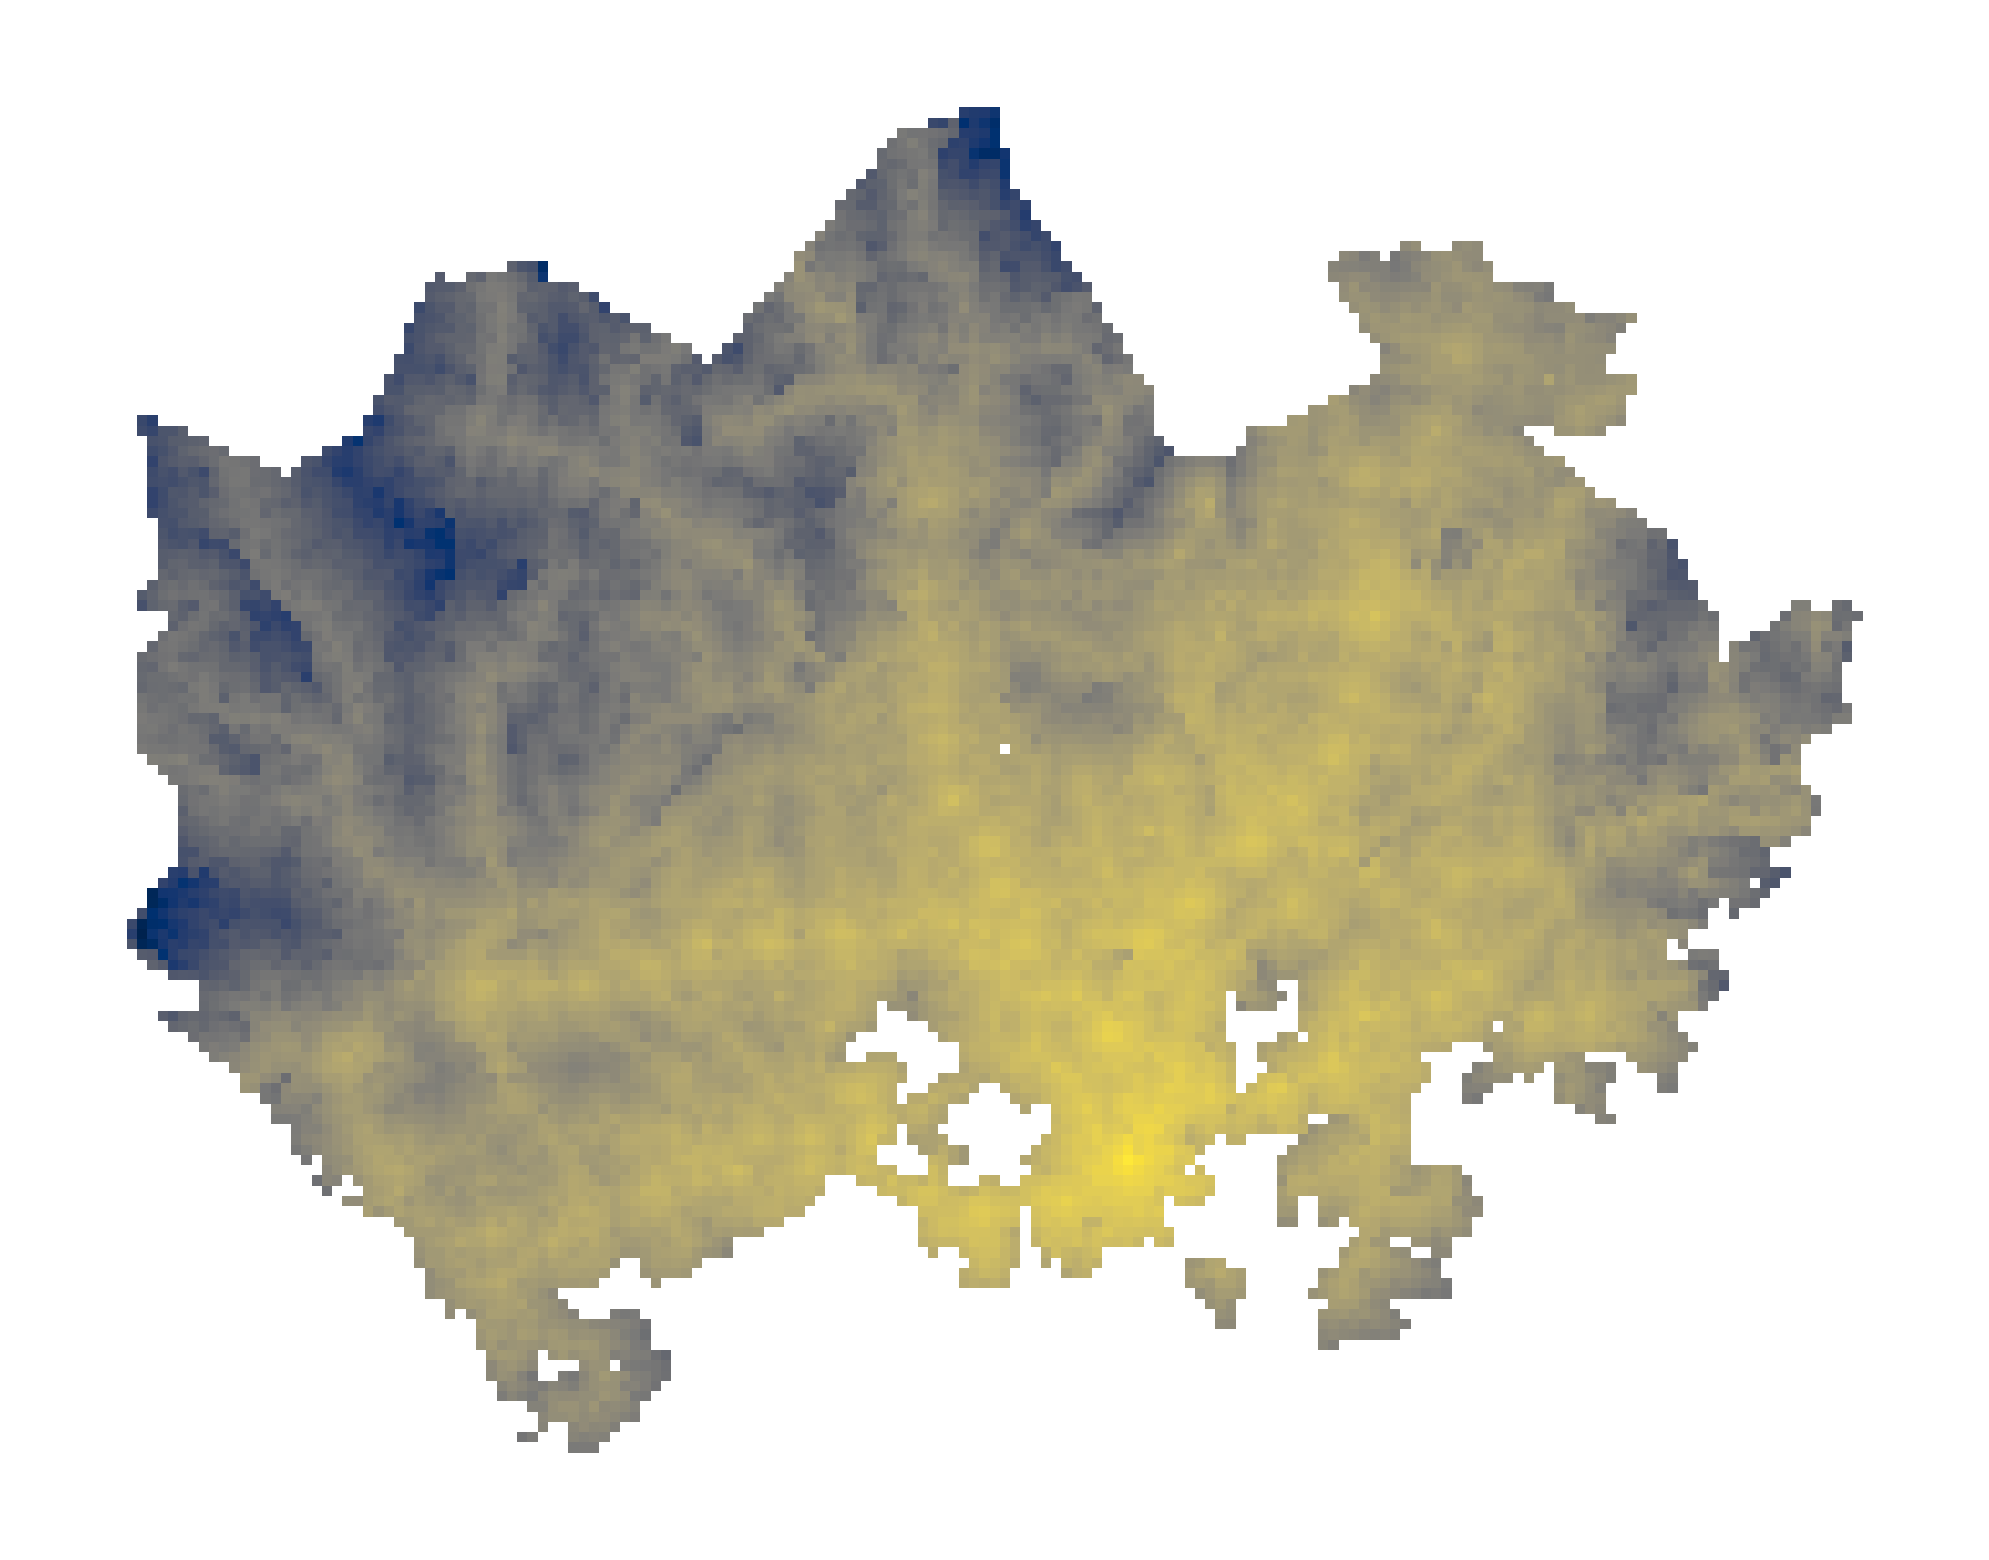
\includegraphics[width=\textwidth]{visual/figures/ttm/isochrone_interval_1}
		\caption{No isochrones}
		\label{fig:interval 1}
	\end{subfigure}%
	\hfill
	\begin{subfigure}[b]{0.5\textwidth}
		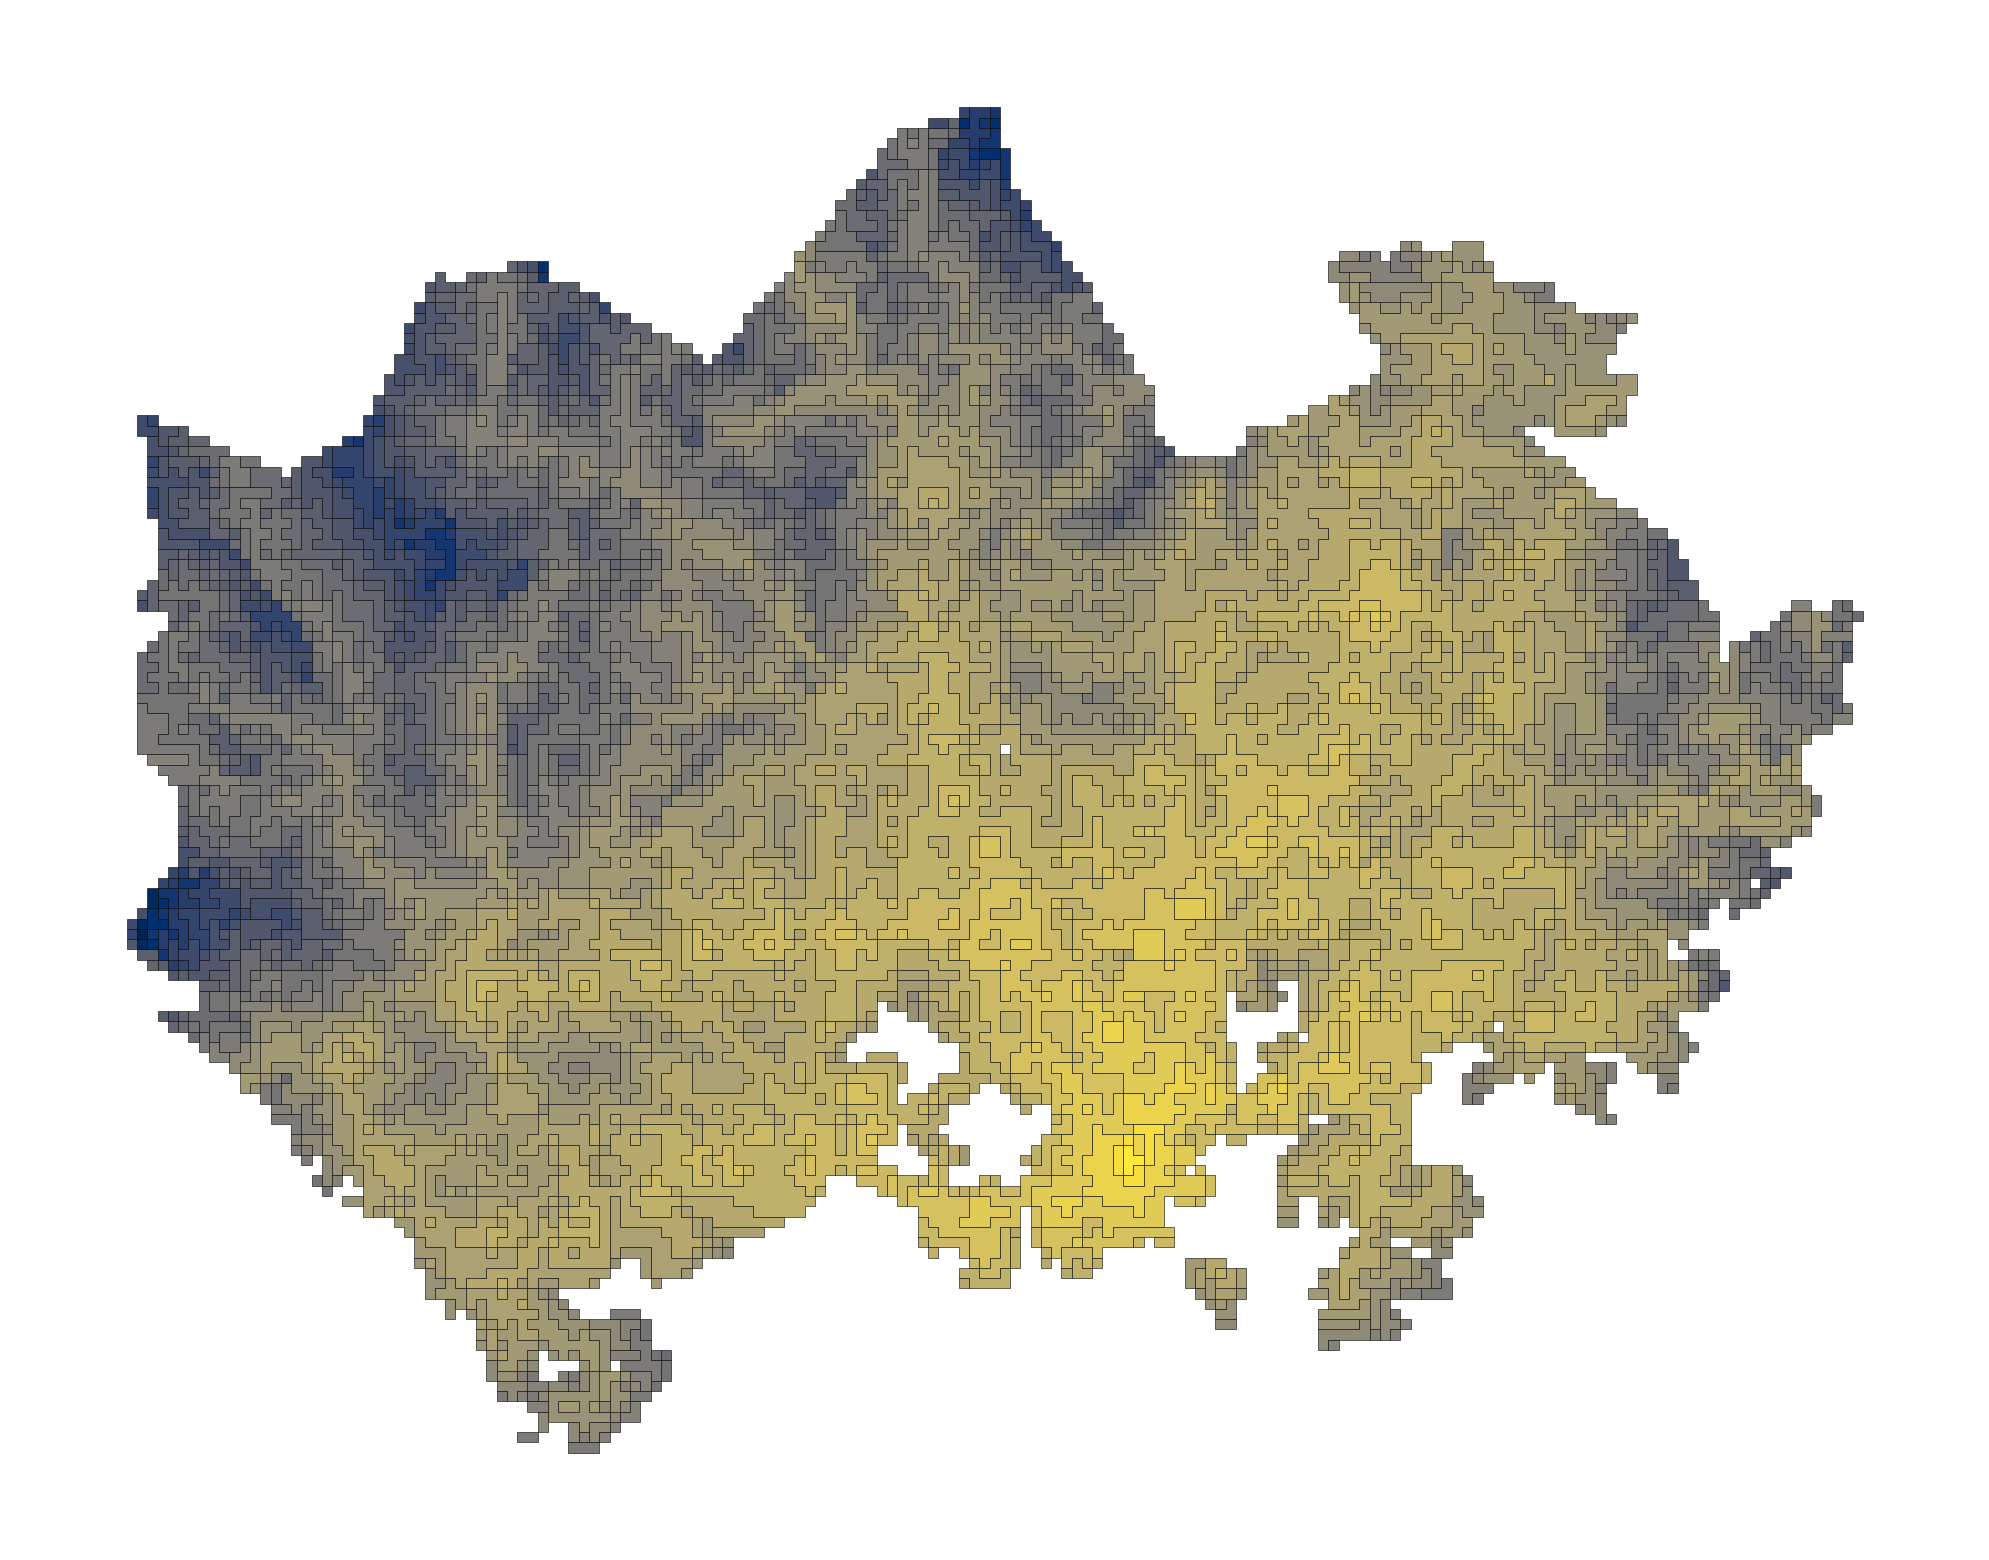
\includegraphics[width=\textwidth]{visual/figures/ttm/isochrone_interval_5}
		\caption{Isochrone interval = 5 minutes}
		\label{fig:interval 10}
	\end{subfigure}%
	\hfill
	\begin{subfigure}[b]{0.5\textwidth}
		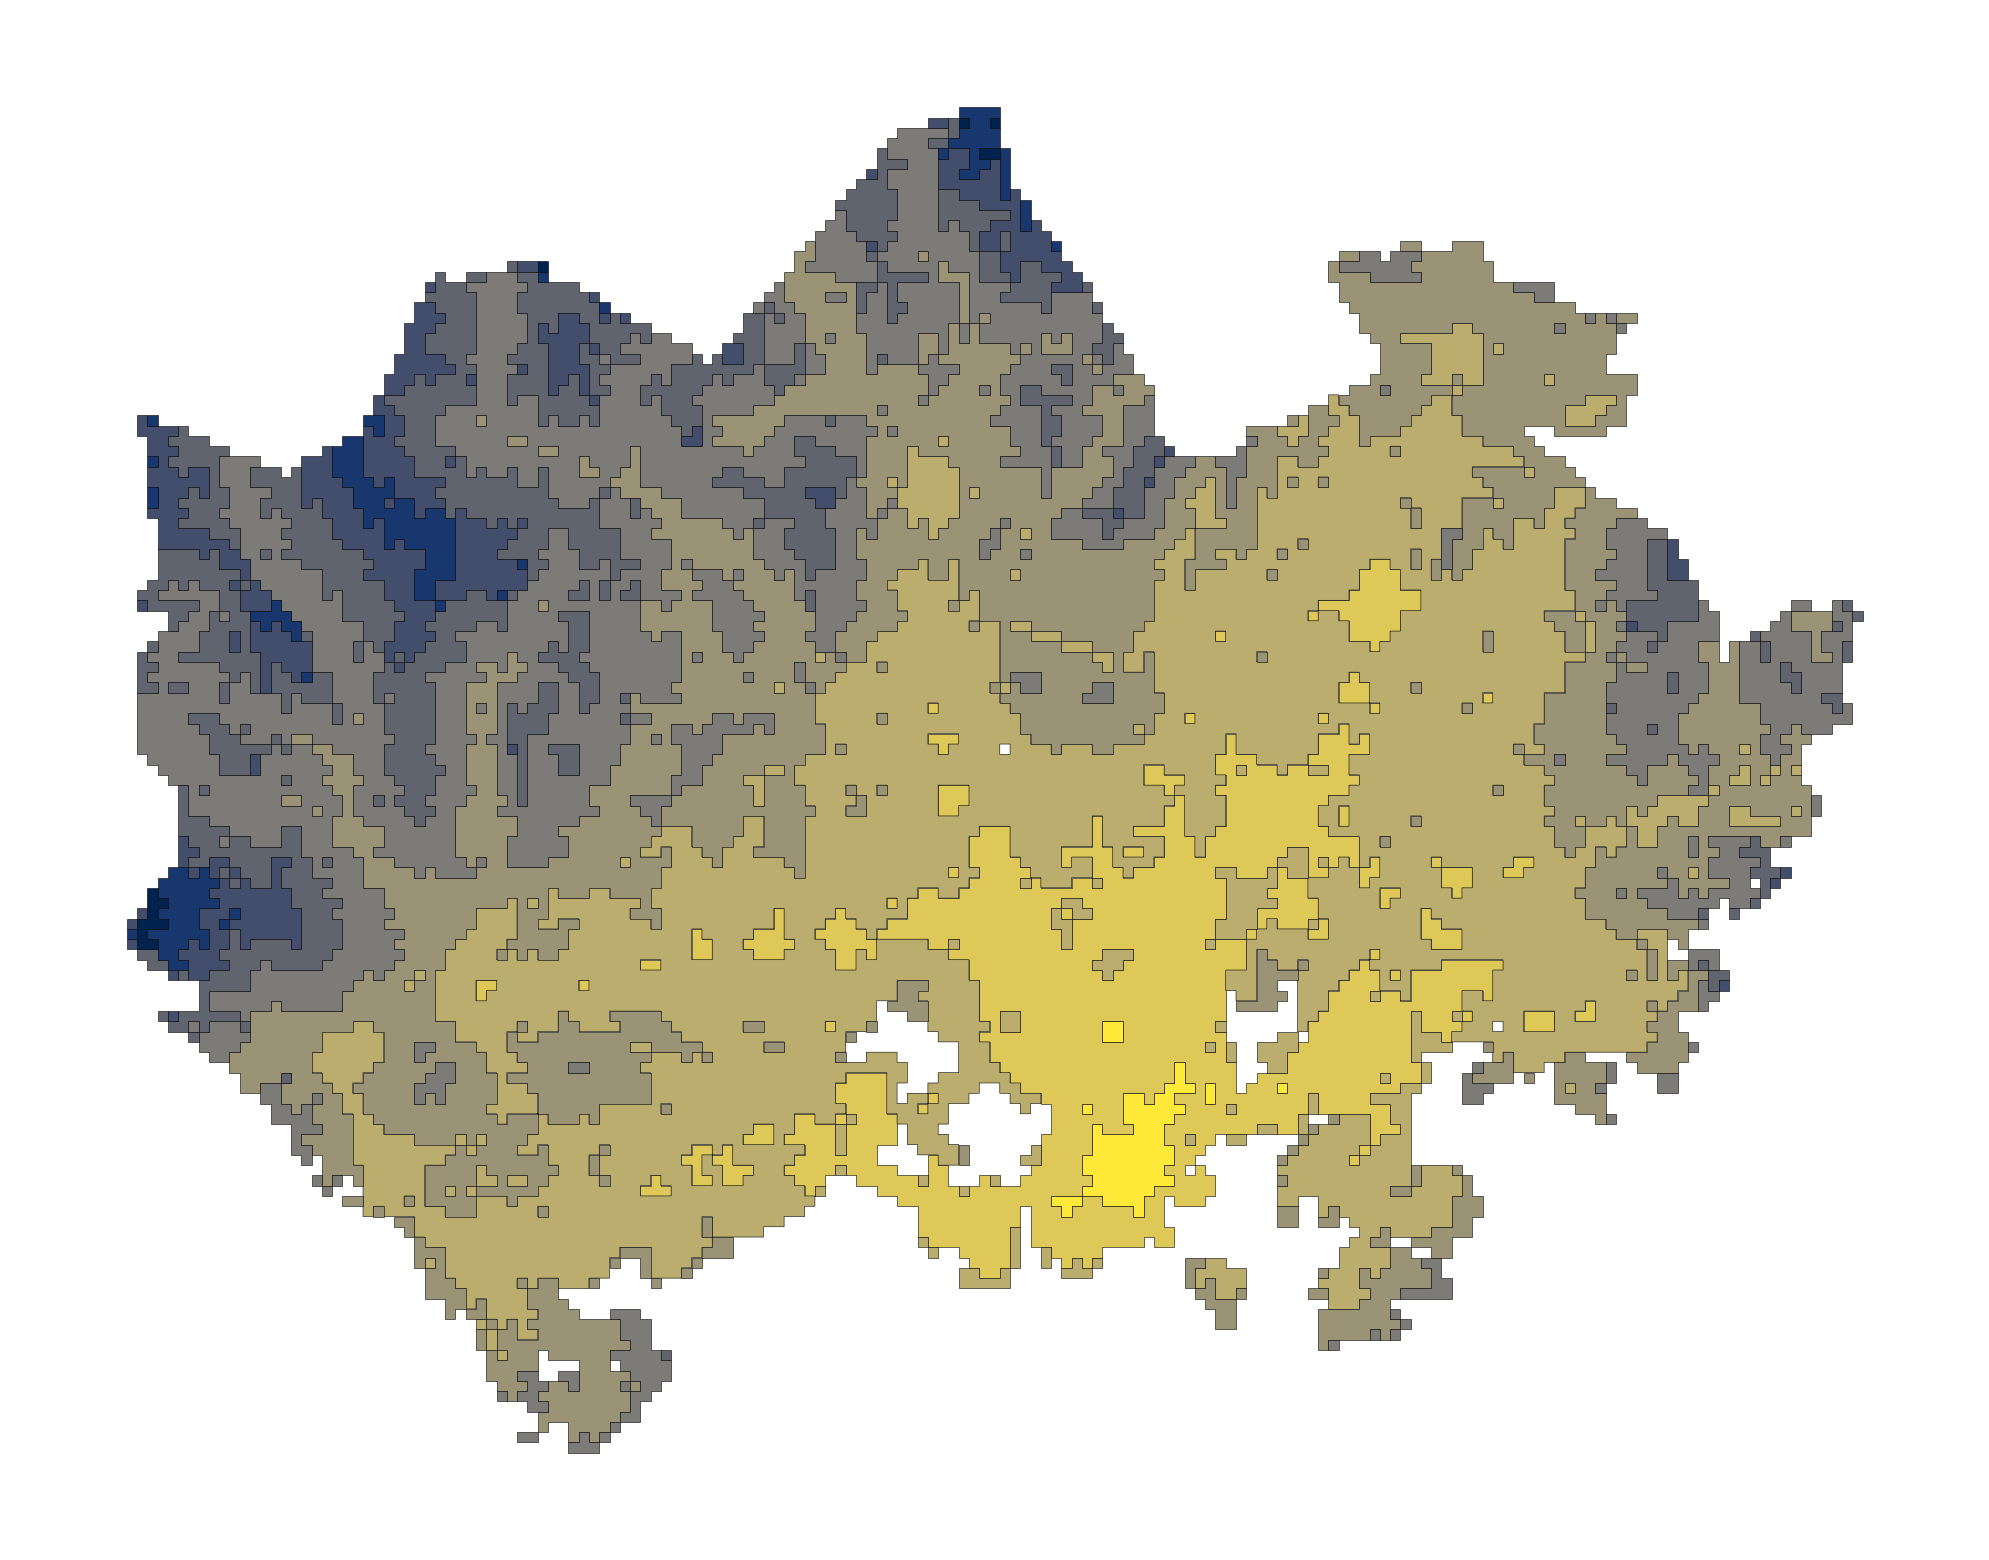
\includegraphics[width=\textwidth]{visual/figures/ttm/isochrone_interval_15}
		\caption{Isochrone interval = 15 minutes}
		\label{fig:interval 15}
	\end{subfigure}%
	\hfill
	\begin{subfigure}[b]{0.5\textwidth}
		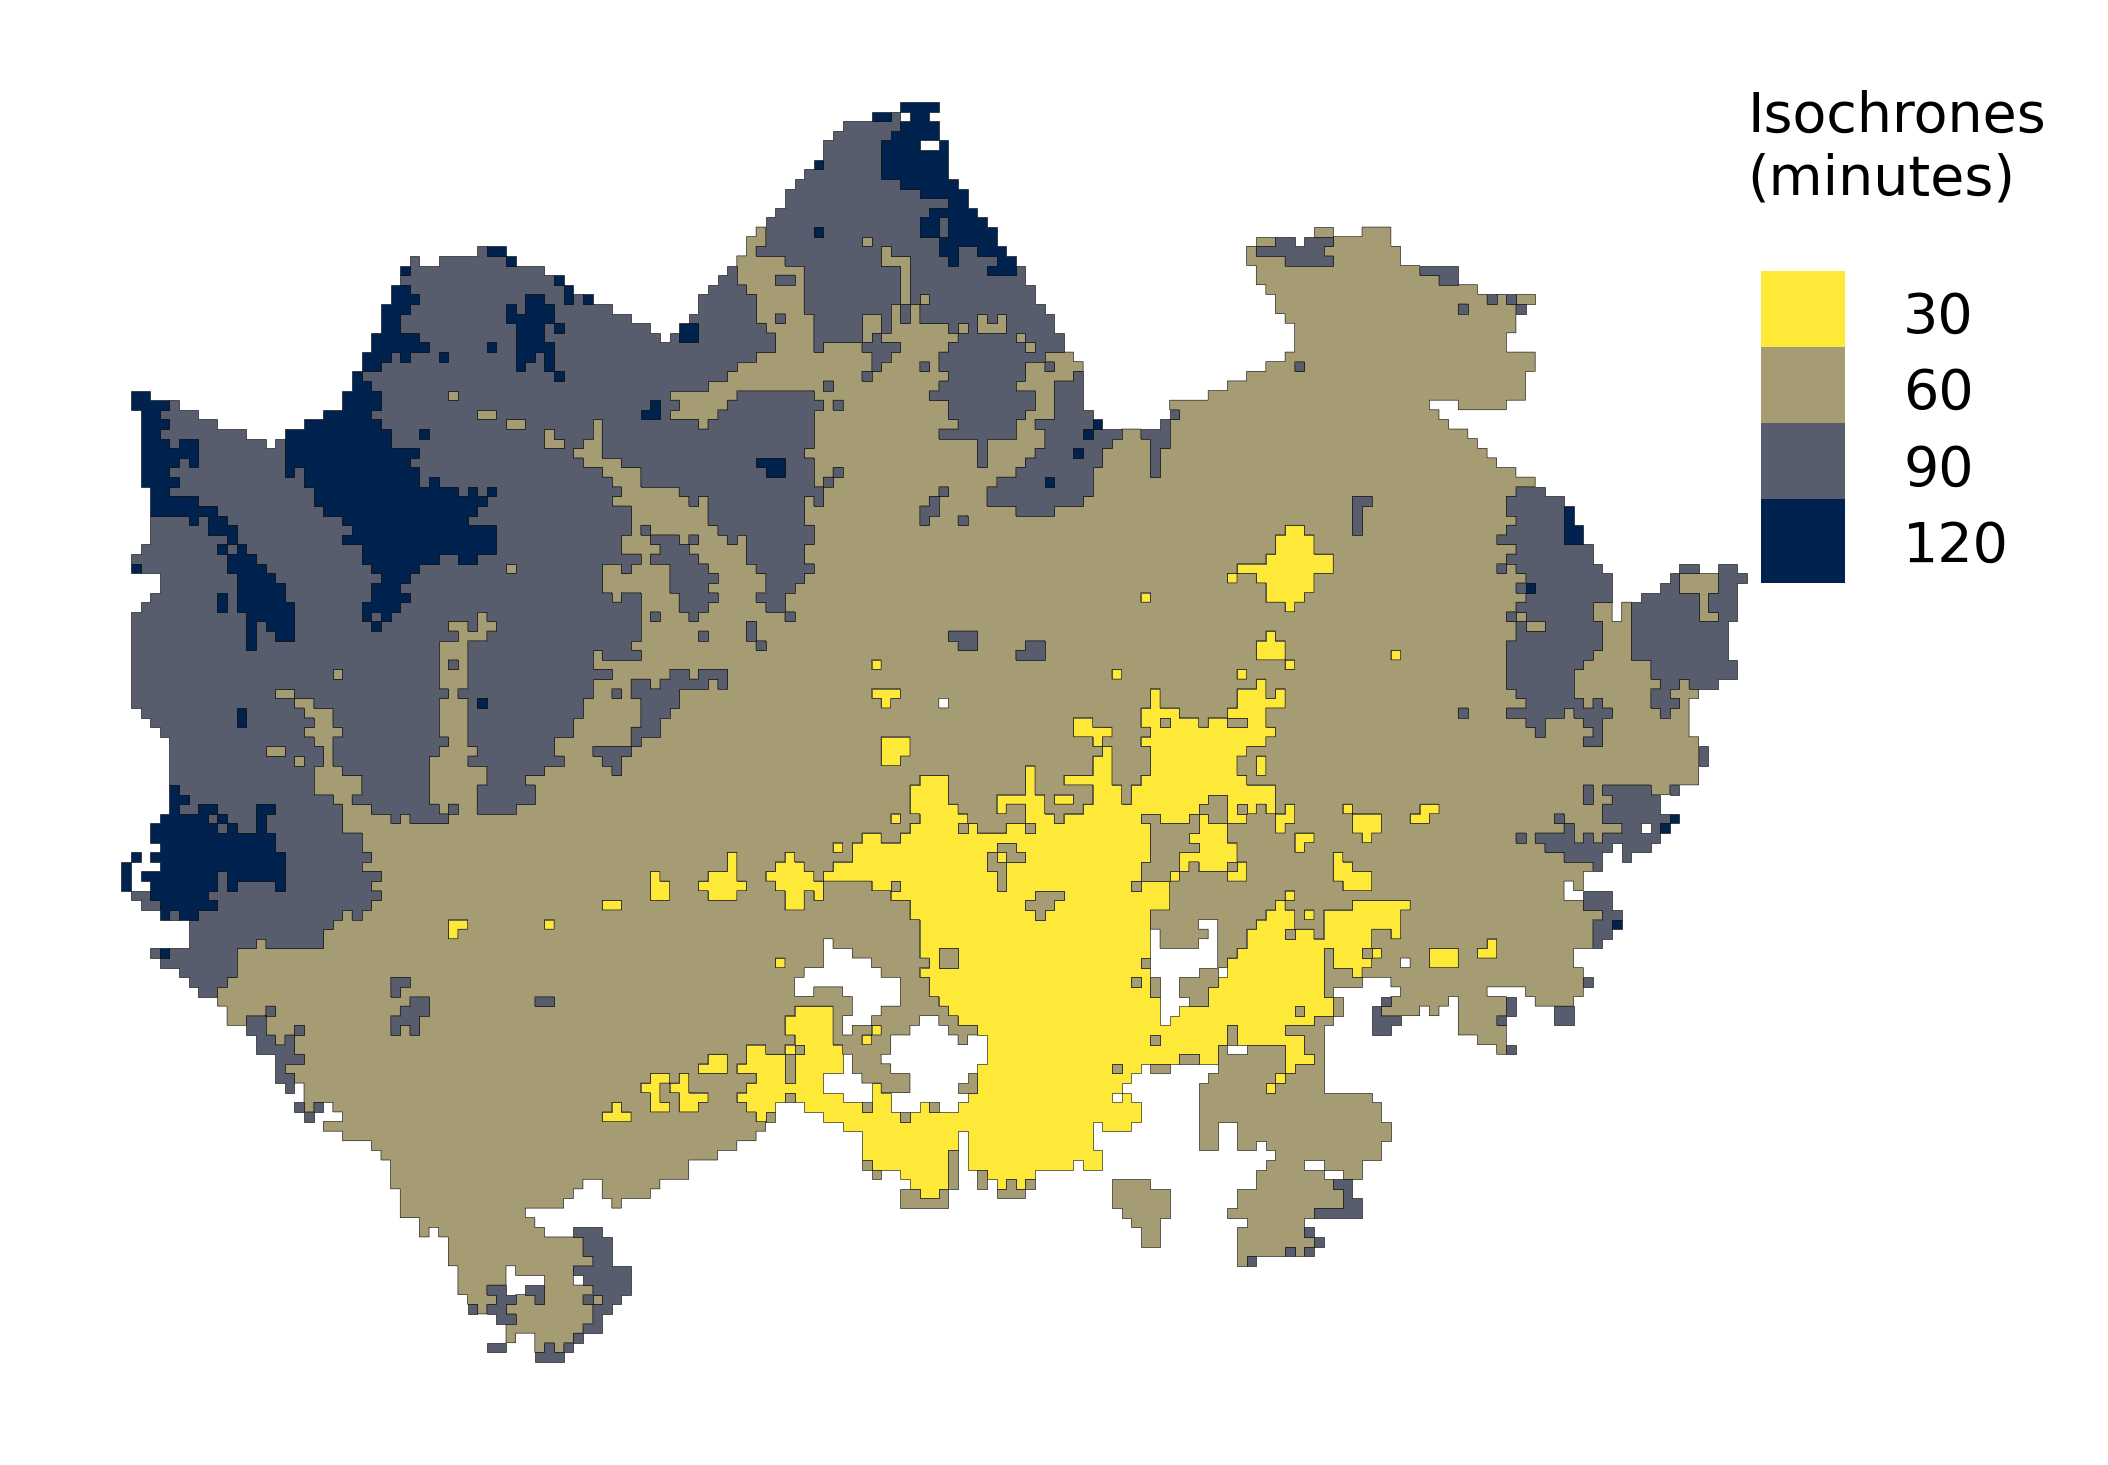
\includegraphics[width=\textwidth]{visual/figures/ttm/isochrone_interval_30}
		\caption{Isochrone interval = 30 minutes}
		\label{fig:interval 30}
	\end{subfigure}%
	\hfill
	\begin{subfigure}[b]{0.4\textwidth}
		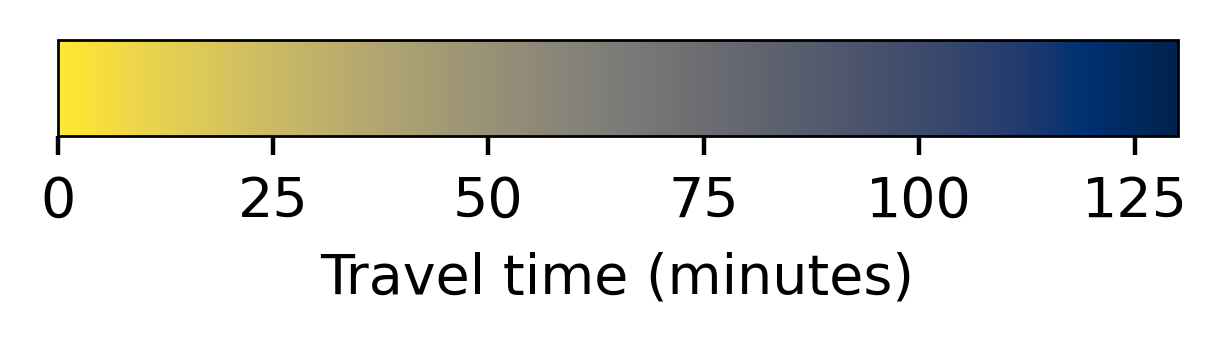
\includegraphics[width=\textwidth]{visual/figures/ttm/isochrone_cbar}
	\end{subfigure}%
	\caption{
		Travel time central Helsinki.
		Different levels of simplification can be achieved by
		aggregating travel times into isochrone polygons.
		Four examples are shown here, from no simplification
		to a highly simplified presentation (\ref{fig:interval 1}--\ref{fig:interval 30}).
	}
	\label{fig:isochrone intervals}
\end{figure}

\begin{figure}[H]
	\centering
	\begin{subfigure}[b]{0.5\textwidth}
		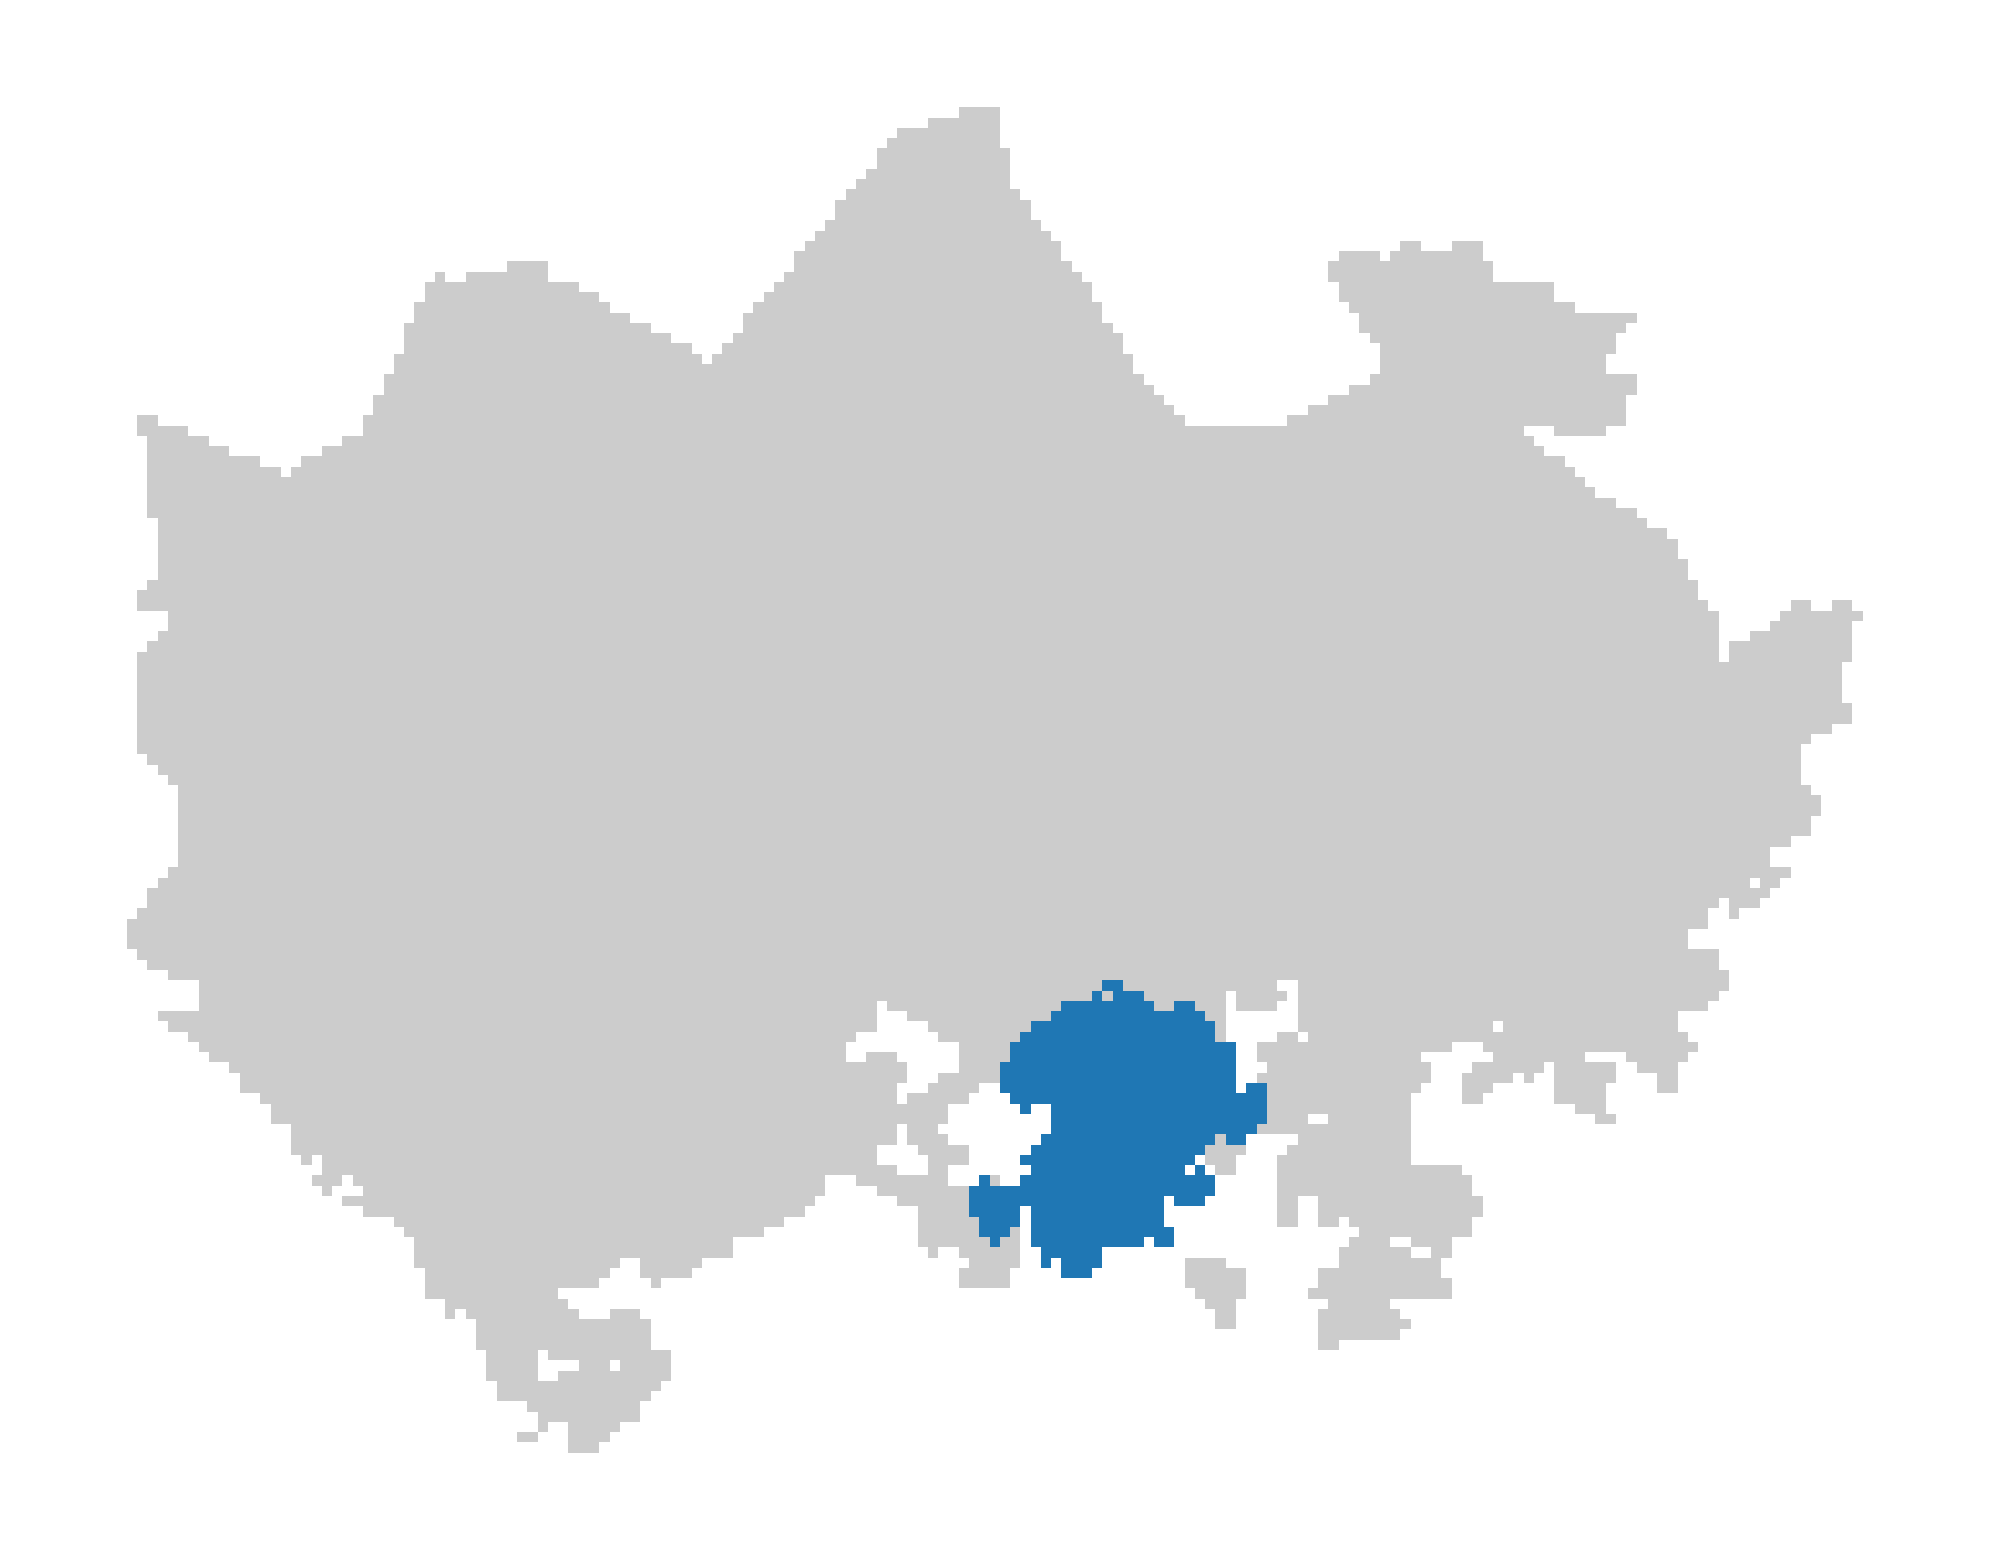
\includegraphics[width=\textwidth]{visual/figures/ttm/tt_limit_walk}
		\caption{Walk, 60-minute limit}
		\label{fig:limit walk}
	\end{subfigure}%
	\hfill
	\begin{subfigure}[b]{0.5\textwidth}
		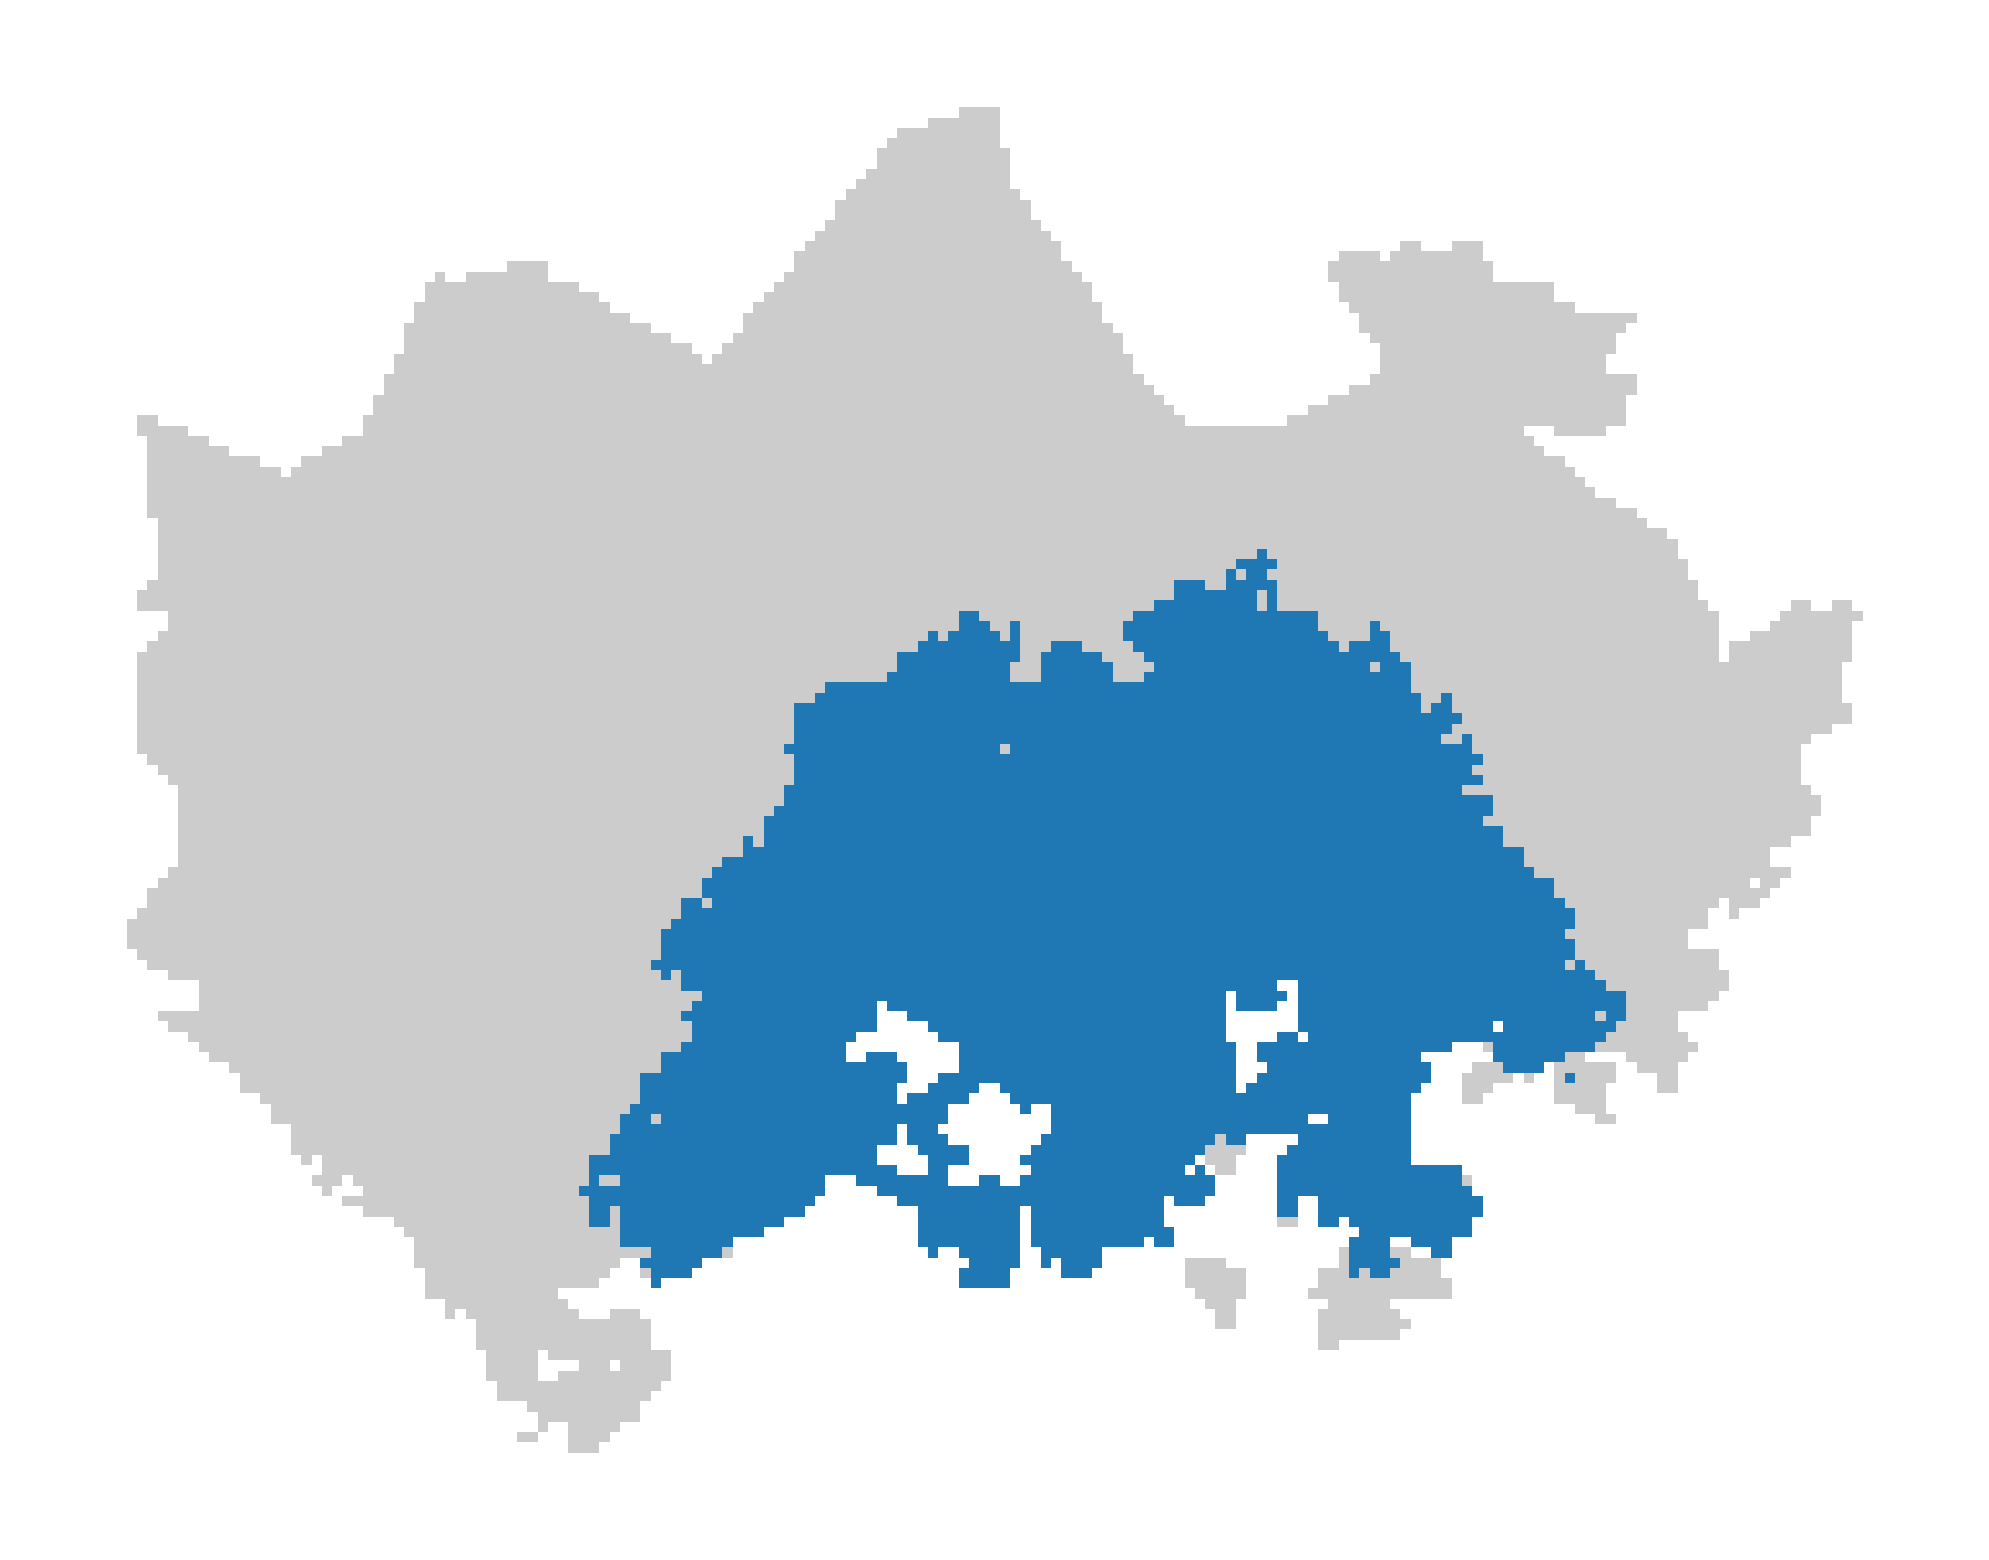
\includegraphics[width=\textwidth]{visual/figures/ttm/tt_limit_bike}
		\caption{Bike, 60-minute limit}
		\label{fig:limit bike}
	\end{subfigure}%
	\hfill
	\begin{subfigure}[b]{0.5\textwidth}
		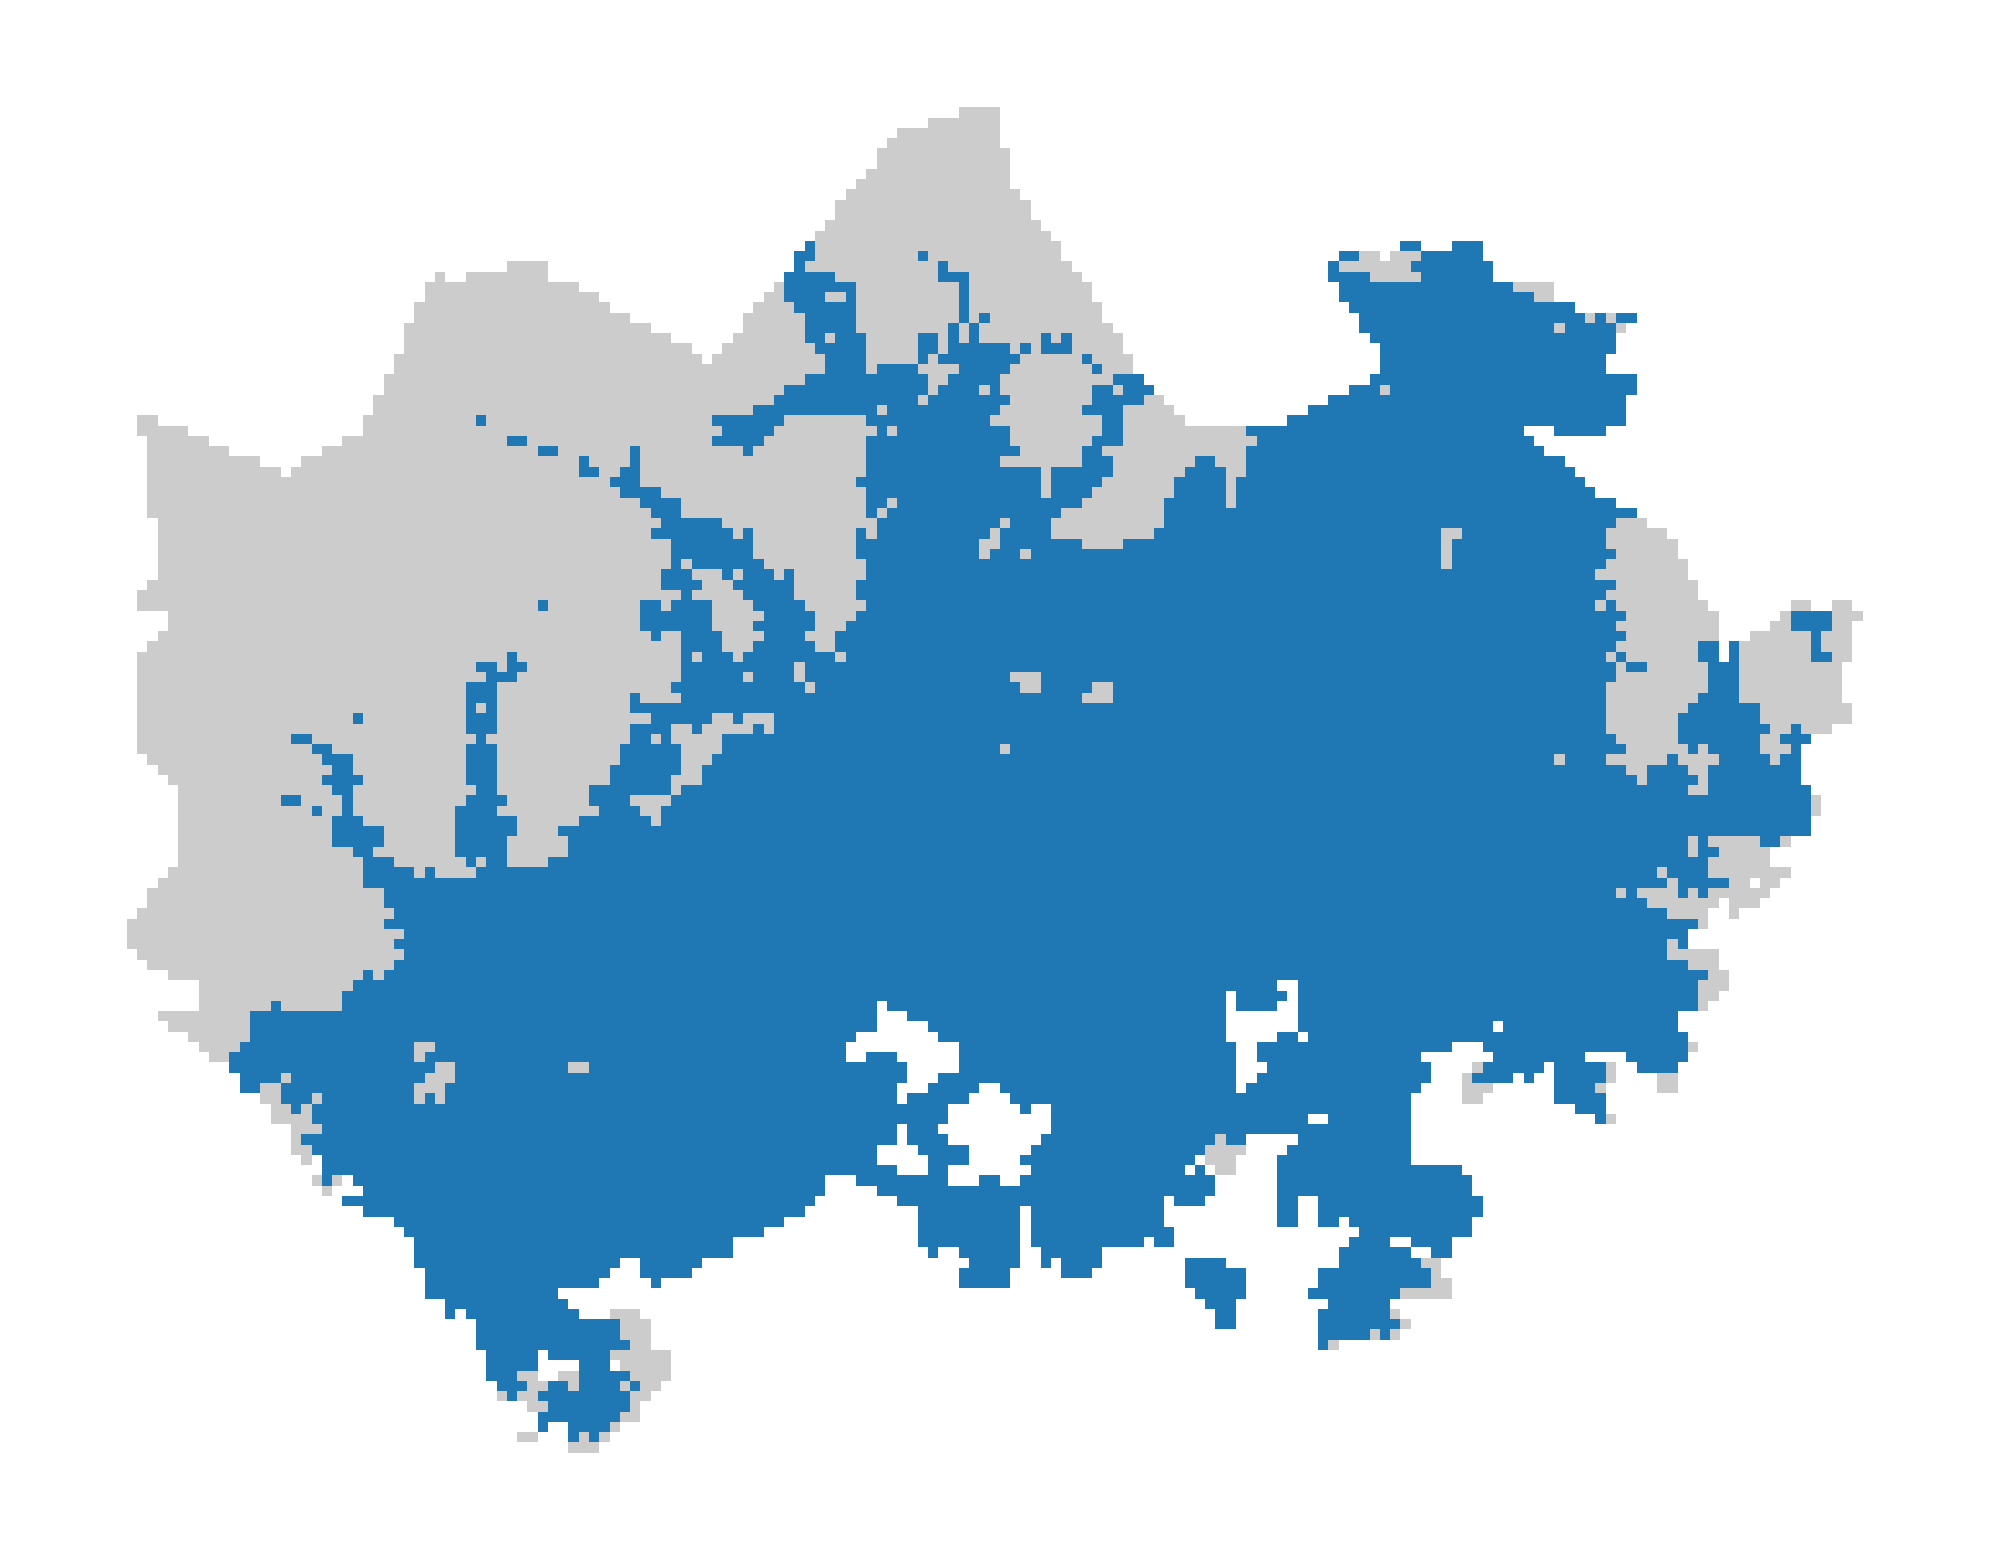
\includegraphics[width=\textwidth]{visual/figures/ttm/tt_limit_pt}
		\caption{Public transport, 60-minute limit}
		\label{fig:limit pt}
	\end{subfigure}%
	\hfill
	\begin{subfigure}[b]{0.5\textwidth}
		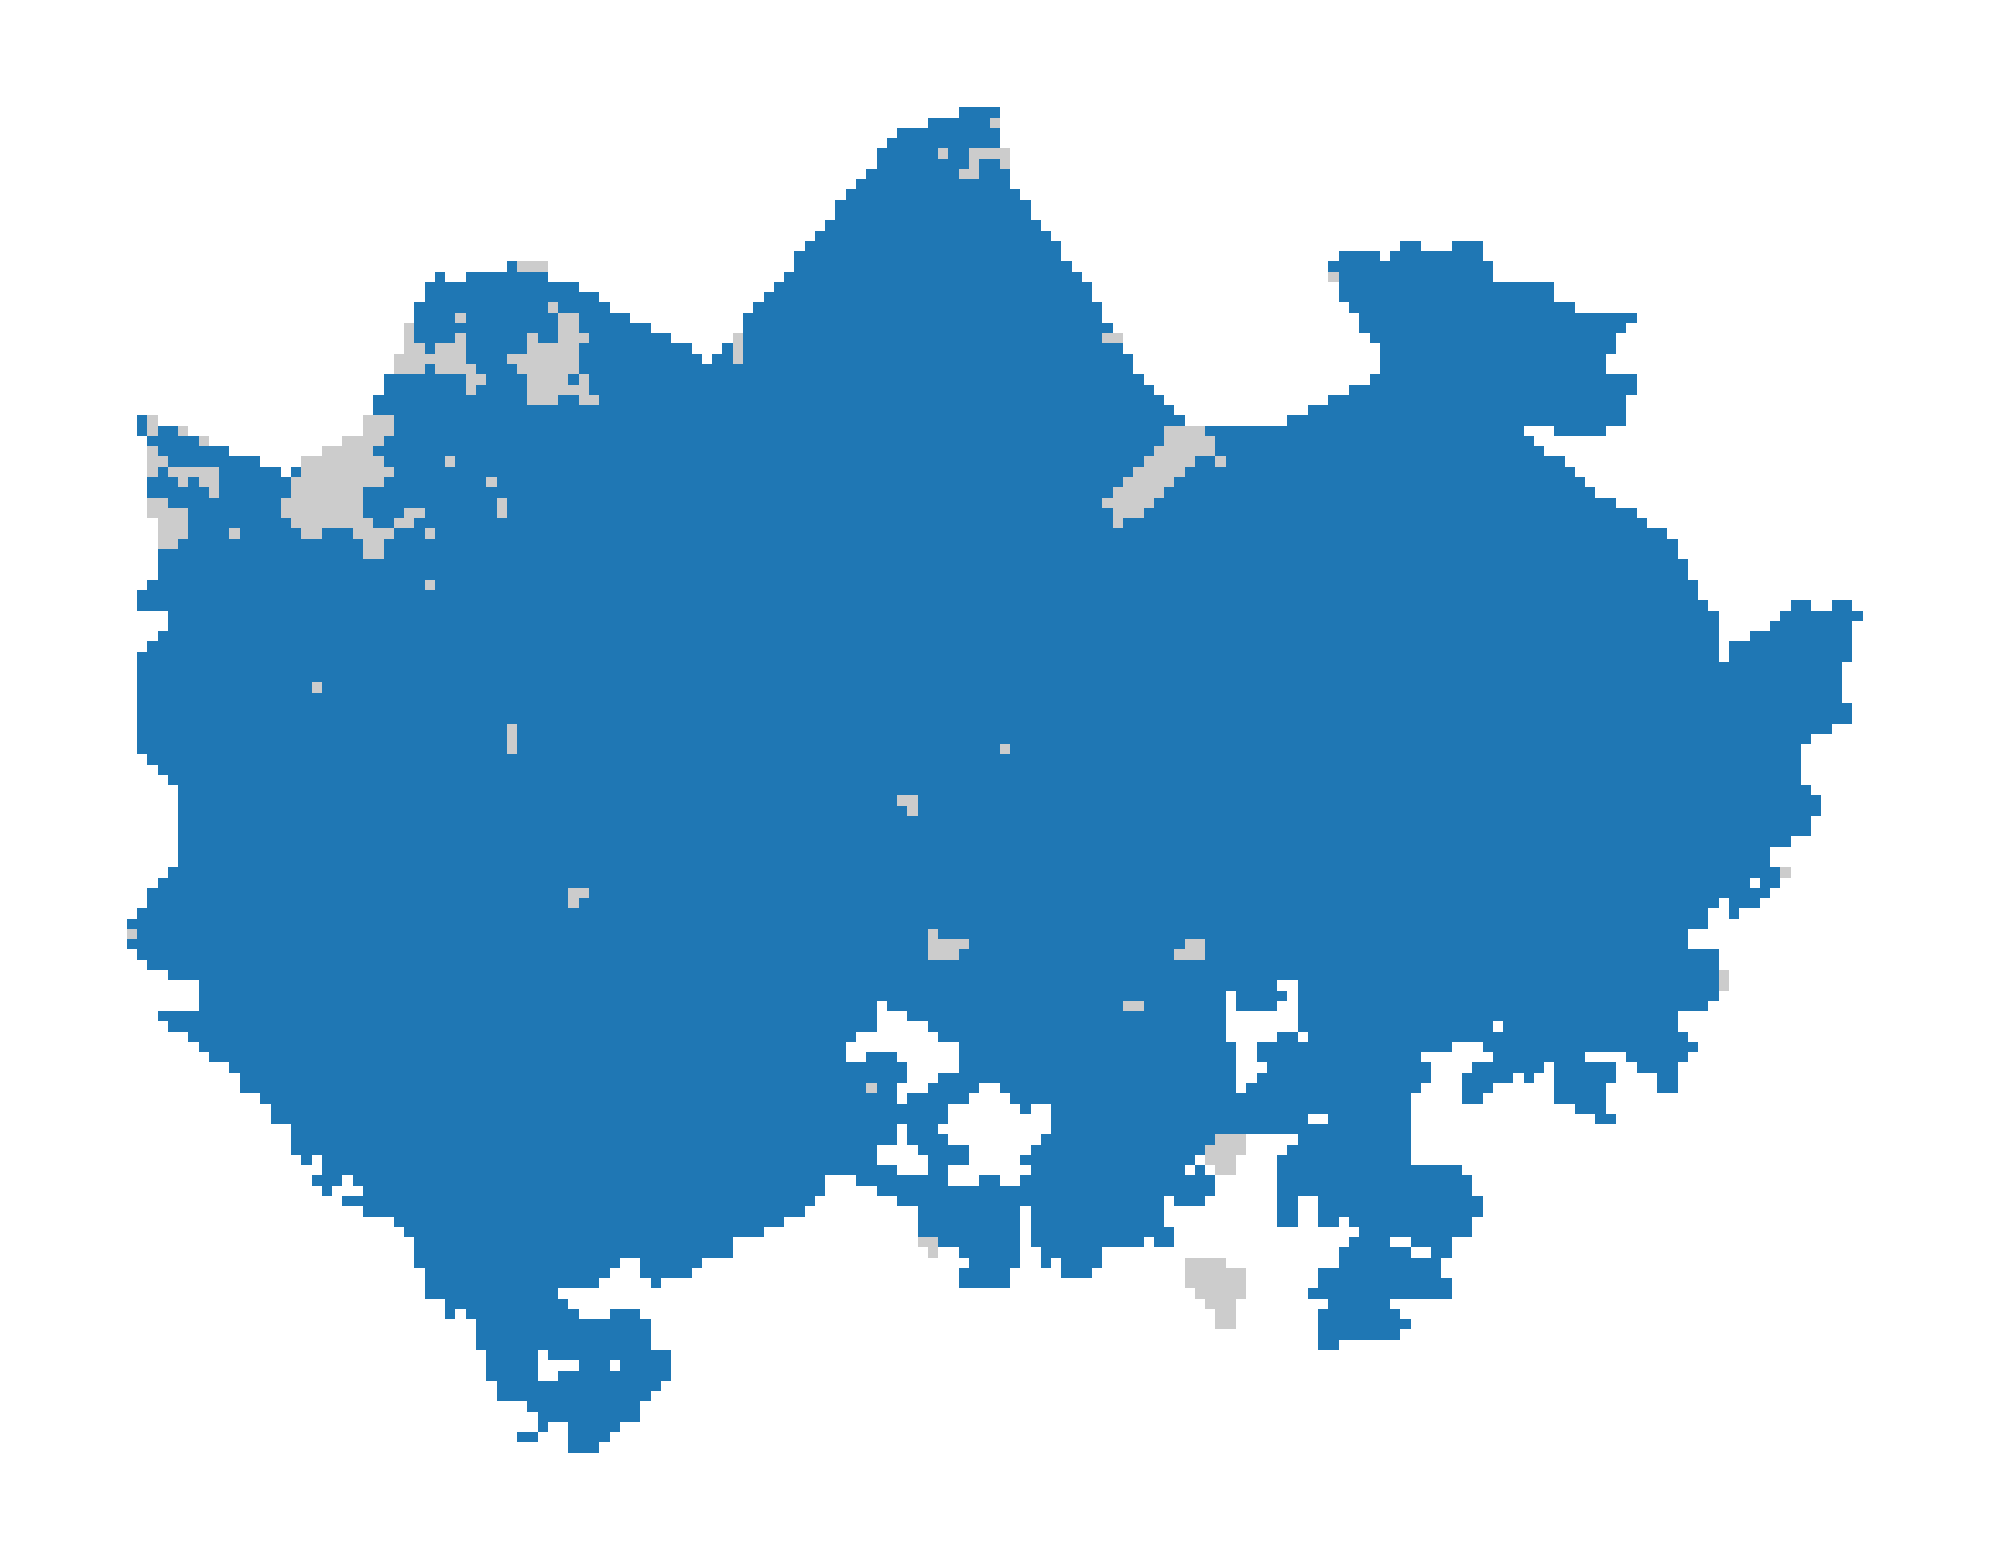
\includegraphics[width=\textwidth]{visual/figures/ttm/tt_limit_car}
		\caption{Car, 60-minute limit}
		\label{fig:limit car}
	\end{subfigure}%
	\hfill
	\begin{subfigure}[b]{0.55\textwidth}
		
\includegraphics[width=\textwidth]{visual/figures/ttm/tt_limit_legend}
	\end{subfigure}%
	\caption{
		The area accessible within an hour of travel from central Helsinki.
		In general, limiting the maximum travel time reduces the spatial extent of data,
		more drastically for walking and biking (\ref{fig:limit walk}--\ref{fig:limit bike}),
		and less so for public transport and car (\ref{fig:limit pt}--\ref{fig:limit car}).
	}
	\label{fig:tt limits}
\end{figure}

To enable the assessment
I constructed a modular preprocessing pipeline
(figure \ref{fig:preprocessing}).
By modular I mean that,
while the complete pipeline applies all preprocessing approaches,
the design allows for isolated testing of the
different components of the pipeline, with different parameters.
I used Python for implementing most of the preprocessing pipeline,
relying on the GeoPandas \parencite{jor2024} library for all spatial operations.
In addition, I carried out file compression with
the standard GNU utilities bash \parencite{bash} and gzip \parencite{gzip}.
Gzip compression was the natural choice,
as it is the ubiquitous approach to file compression on the web. 
I tested the preprocessing approaches on
a randomly picked set of 100 locations in the \acrshort{ttm},
for each travel mode.
A random sample of locations is necessary when either
isochrone aggregation or a travel time limitation is applied,
since in these cases the complexity of the resulting
data varies greatly based on location.

\begin{figure}[H]
	\centering
	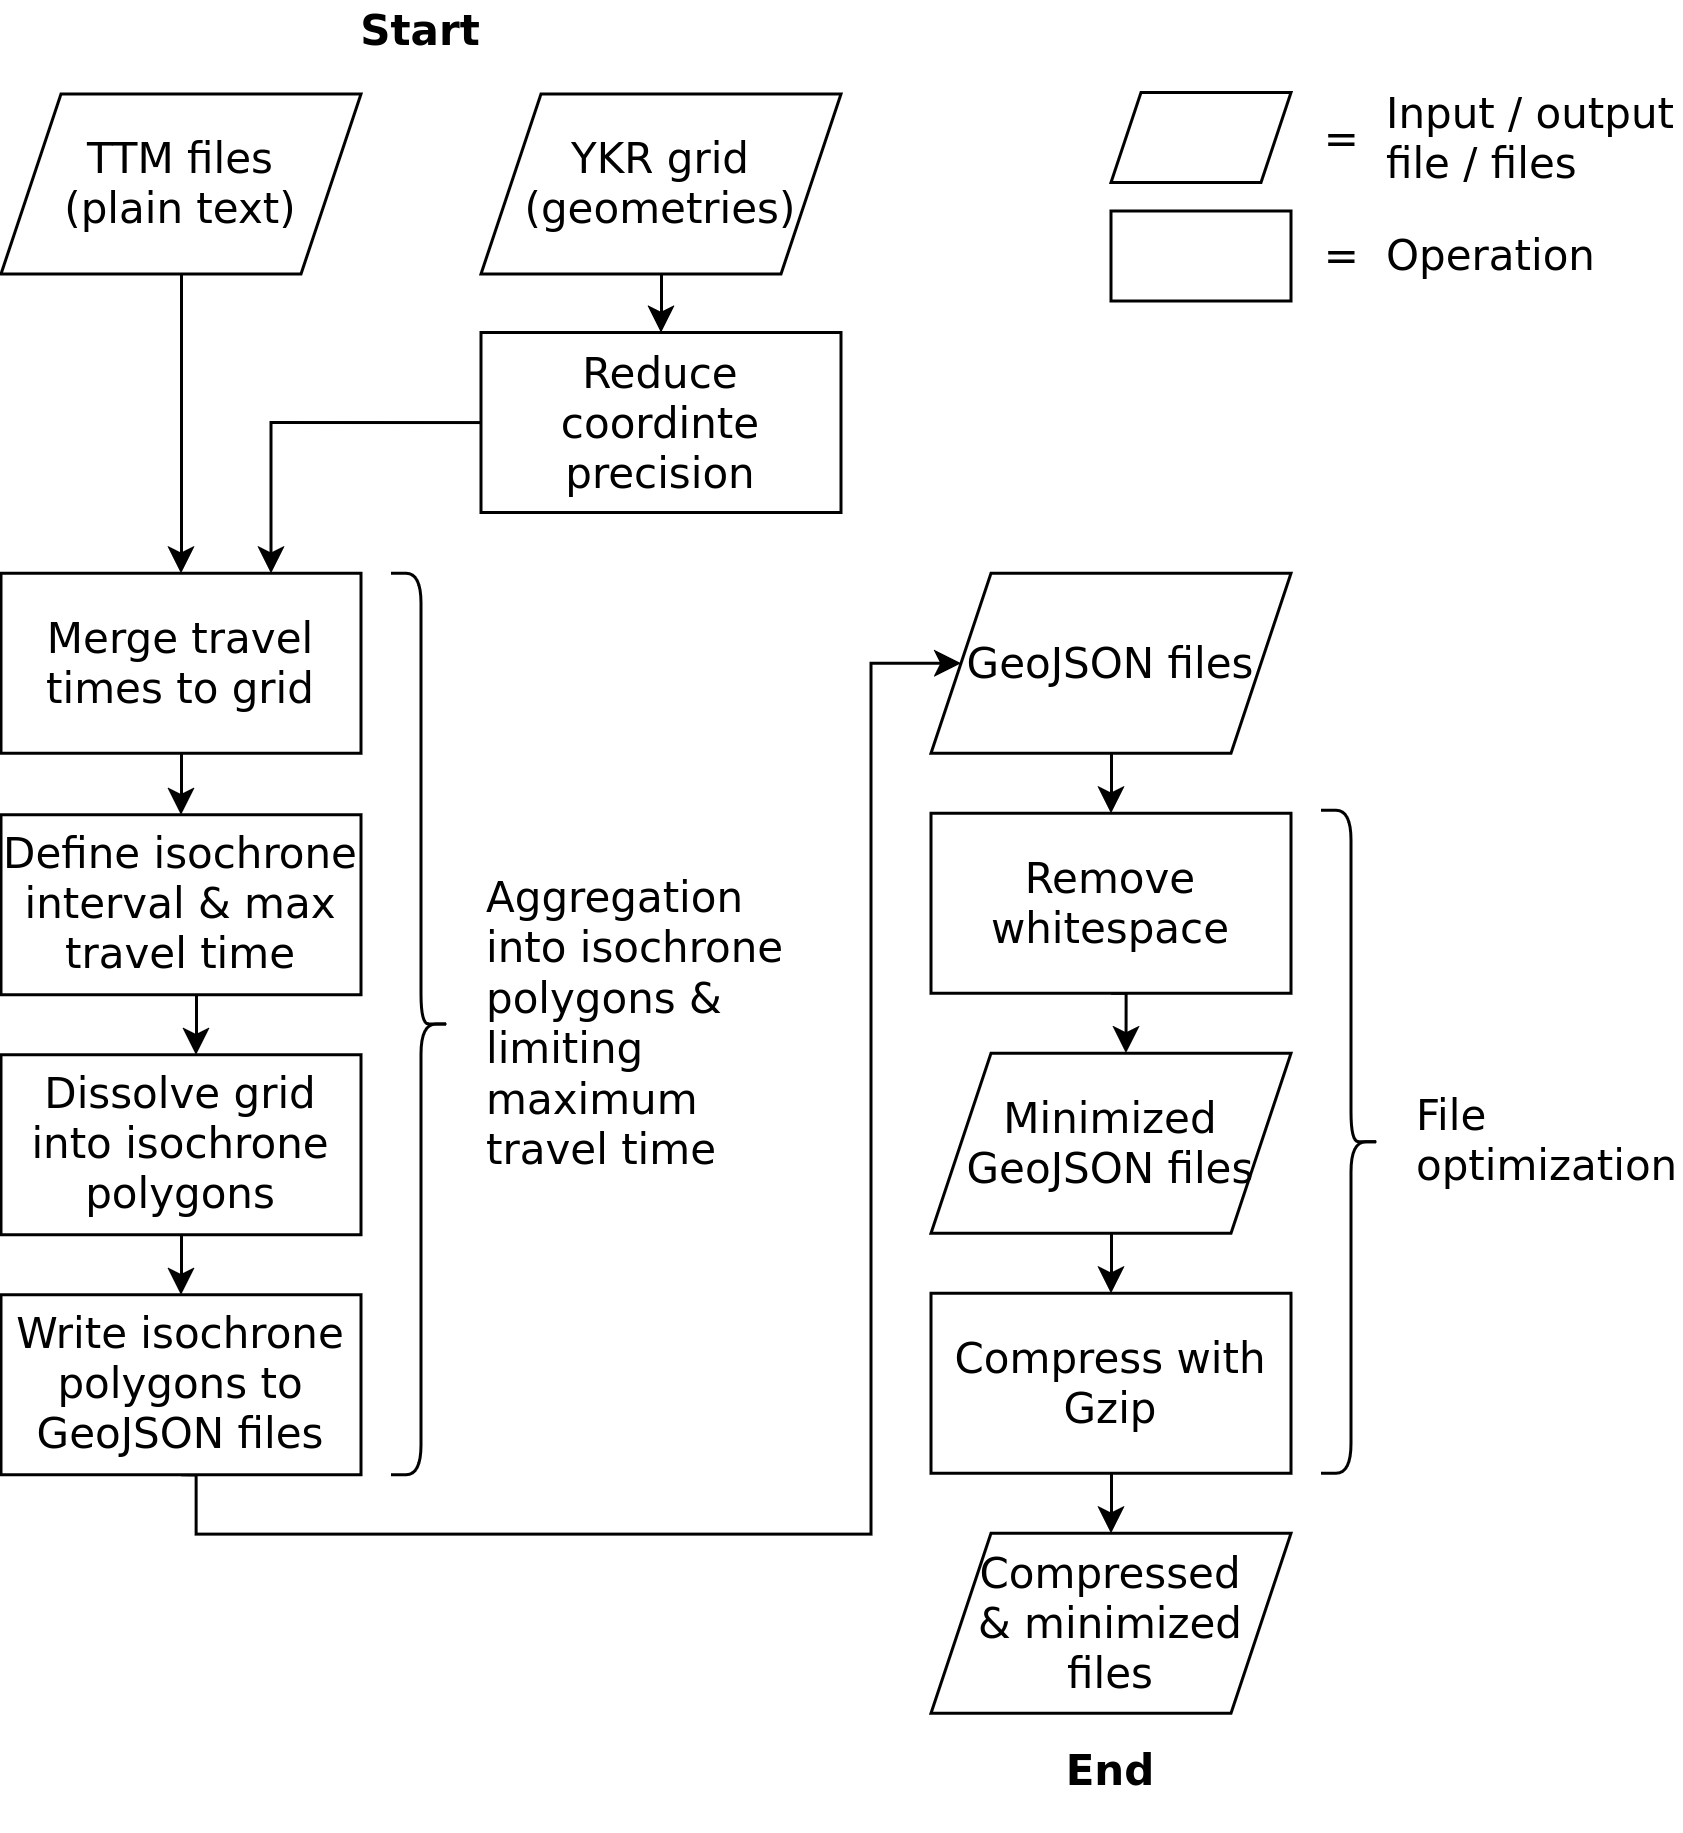
\includegraphics[width=\diagramwidth]{visual/figures/diagrams/preprocessing.png}
	\caption{Preprocessing}
	\label{fig:preprocessing}
\end{figure}

To measure the effects on file sizes,
I calculated the mean combined file size of the all the files needed to represent
all the travel modes for a single cell in the dataset
when a given approach has been applied.
I calculated these values as averages of a random sample as described above.

I assessed the impact the preprocessing approaches have on rendering speed
by using the data with the finished map application.
The details of the map application are in the next section.
This assessment was qualitative,
as it was based on my own perception of responsiveness when using the map.
Quantitative testing of rendering speed would have been preferable,
but it proved to be difficult.
While many tools for profiling the rendering speed of web applications exist,
I did not succeed in two main areas
that would have been necessary for representative results.
I did not manage to limit the timing to strictly the map
component of the interface in such a way that
the test results would be reproducible.
I also did not find a way to automate a set of renders
on a sample of locations.
Averaging the renders of a single location would not suffice
due to the differences of data complexity between locations.
The tools I tried were the Firefox profiler
and the React developer tools browser extension on Firefox and Chromium
(I'll need to properly refer to these).

I carried out the assessment of loss of information in two ways:
Qualitatively for all approaches by observing the processed data on the map,
and, in the case of limiting maximum travel time,
quantitatively by calculating the percentage of the total dataset area
that the processed data covers.
These percentages are, again, averages of a random sample as described above.

Appendix \ref{appendix:repositories} includes a link to the repository
containing the preprocessing pipeline.
The same repository also holds the quantitative tests described above
as an interactive Jupyter Notebook.

\subsubsection{Assessing web mapping libraries}

The solution for rendering the data to a map, i.e. the web mapping library,
was one of the most important decisions of the development process. 
In addition to rendering data correctly and efficiently,
the mapping library must allow for user interaction not only with the map,
but the underlying application.
Often, interaction with a web map changes only the state of the map,
for example by zooming,
and the web-mapping library handles an internal state change like this automatically.
With the map presentation I developed,
the map interaction must also change state outside the map.
For example:
Location selection should result in the fetching of new data from the backend,
and the mode of map interaction must be changed by map interaction.

\begin{figure}[H]
	\centering
	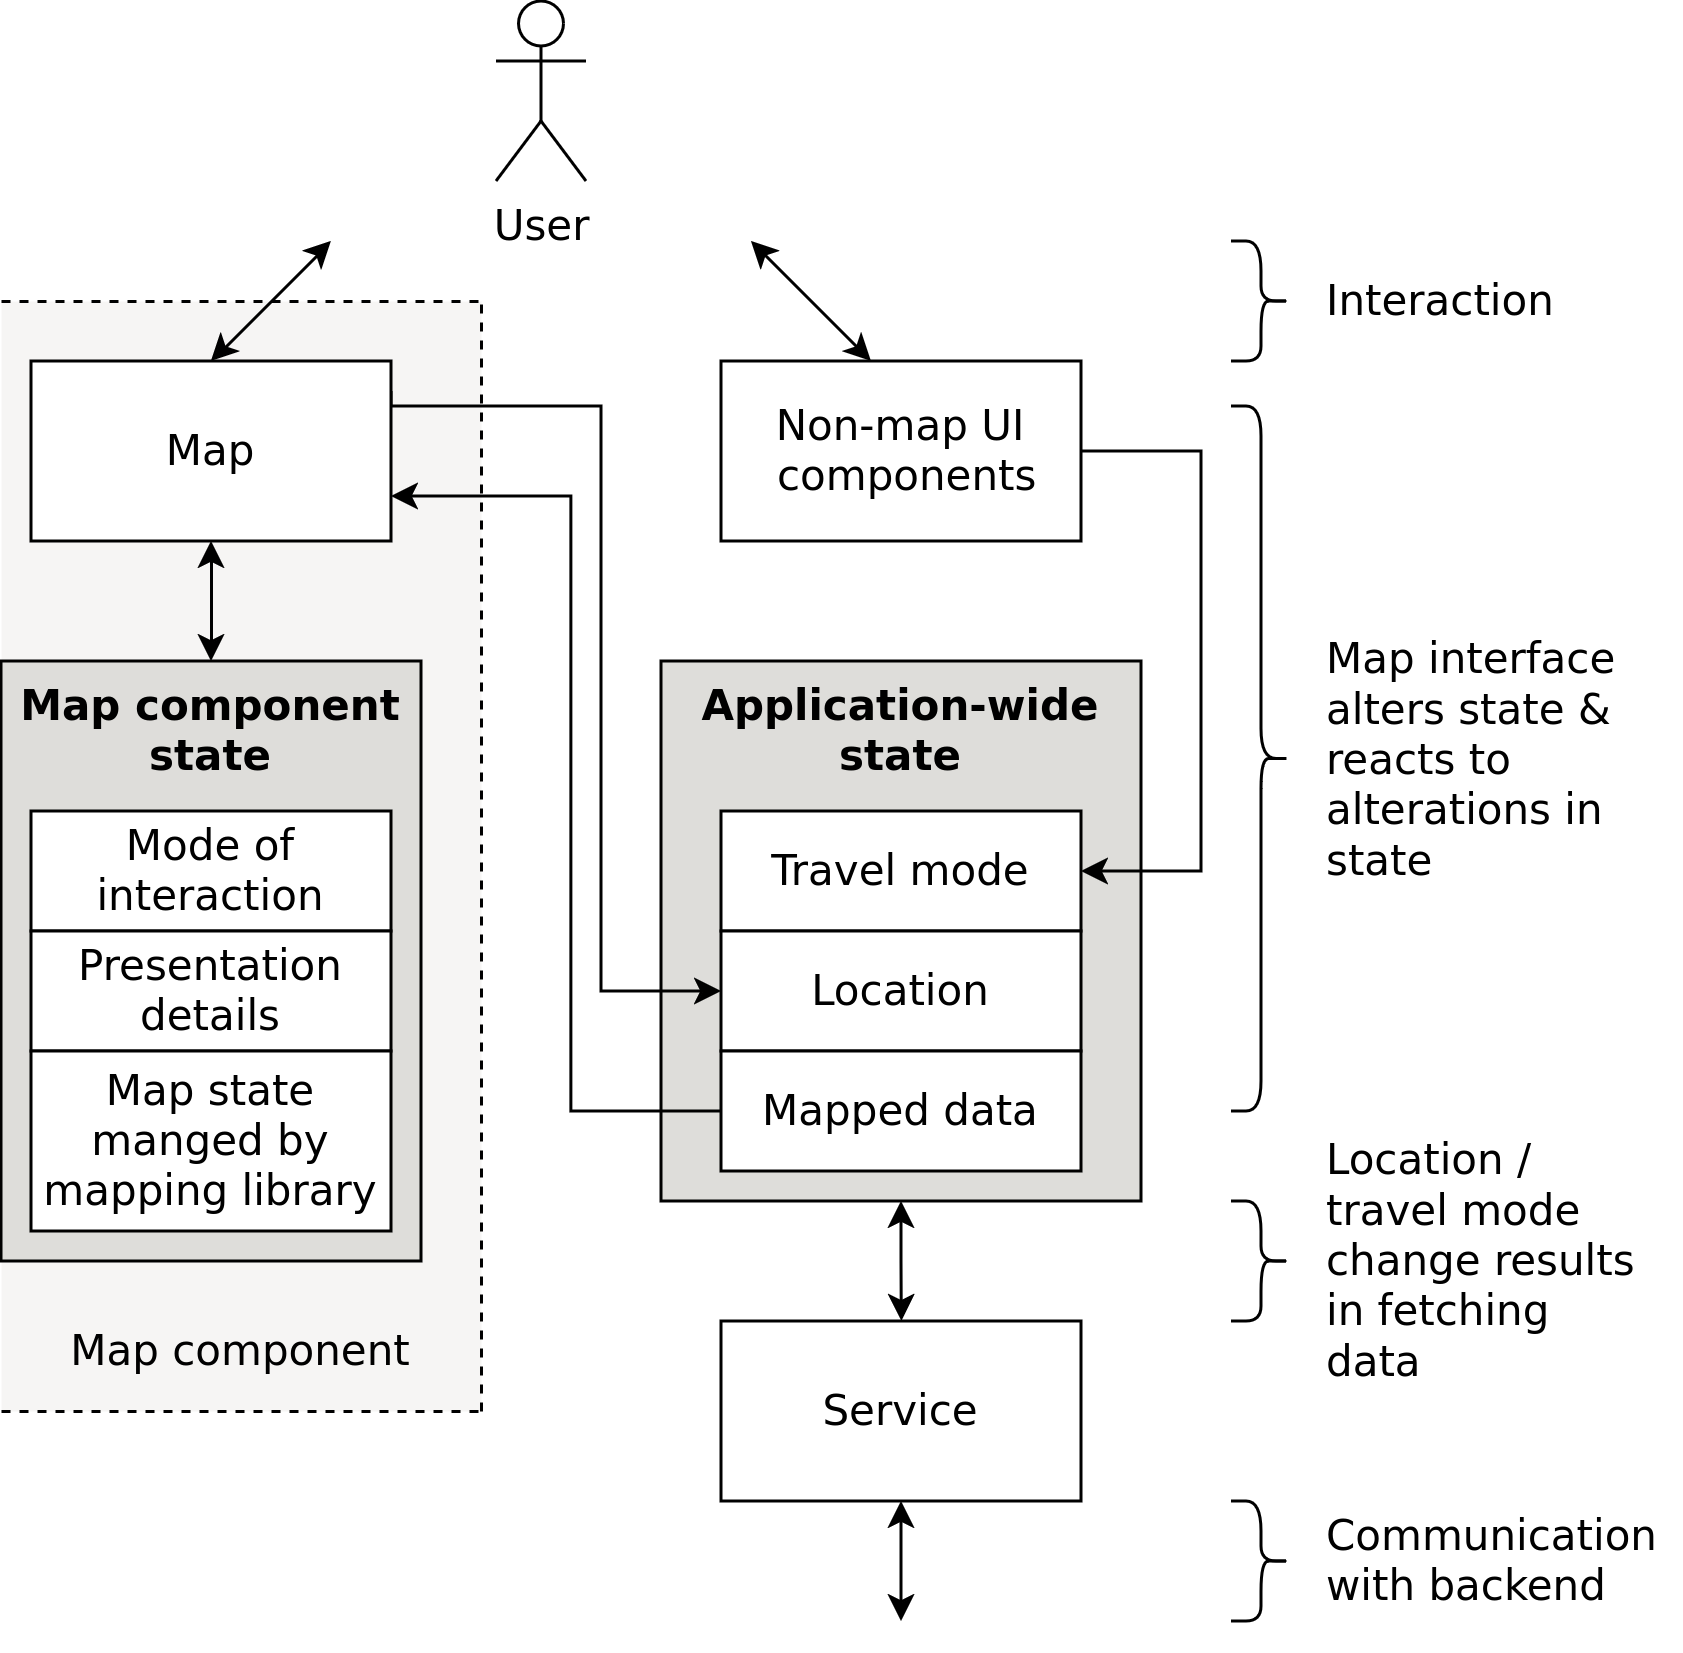
\includegraphics[width=\diagramwidth]{visual/figures/diagrams/frontend.png}
	\caption{Frontend}
	\label{fig:frontend}
\end{figure}

Controlling state in web-applications is often best done by a specified solution,
such as a state store or, if applicable, a UI framework.
For this map presentation I chose to control application state with React,
as it is the most widely used and documented UI framework,
and also the only UI framework that many web-mapping libraries have integration capabilities for.
In general, integration with a framework instead of a self-made solution
means less room for error in the implementation,
and better maintainability and extensibility as the amount of code is drastically smaller.
Also, I used React in implementing the few non-map user-interface elements
(travel mode selection, legend, tooltip),
which meant no additional dependencies.

I based my assessment of web mapping libraries on three criteria:
\begin{itemize}
	\item Visual quality of the map
	\item Responsiveness of the map
	\item Integration with React
\end{itemize}

SIDENOTE: I don't know if I should be so technology-specific with React.
React really isn't the point, the point is that a UI framework is sensible
to not have to do everything from the ground up. React just happens to
be \textit{the} framework
(and the only framework pretty much any mapping library integrates with in any way).

When selecting which web mapping libraries to assess, I used the following properties as a baseline:
\begin{itemize}
	\item Free and open source licensing
	\item Actively maintained
	\item At least some level of integration with React
\end{itemize}

With these considerations I arrived at three potential libraries:
Leaflet, Maplibre and Deck.gl.
To assess the criteria above,
I used each library as the map interface with the application.
I assessed visual quality of the map qualitatively, and, for the reasons I stated in the previous chapter,
I had to resort to qualitative assessment for rendering performance as well.
For assessing integration with react additionally I utilized online documentation of potential solutions.

% % TODO copypasta
% Translucent Overlay (OV) is the best technique over-
% all, which makes it a good choice when only one comparison
% technique should be provided to user \parencite{lob2015}.


\subsubsection{Technical infrastructure}

\begin{itemize}
	\item Backend: Minimal HTTP sever serving pre-compressed geojson files directly from filesystem
	\item Scalable Kubernetes / OpenShift deployments → Reproducibility at the level of the entire application
	\item Containerization → Reproducibility at the level of the components of the application
	\item Modularity of the design
	\item the list goes on, I'll have to consider what matters and what doesn't.
\end{itemize}

\begin{figure}[H]
	\centering
	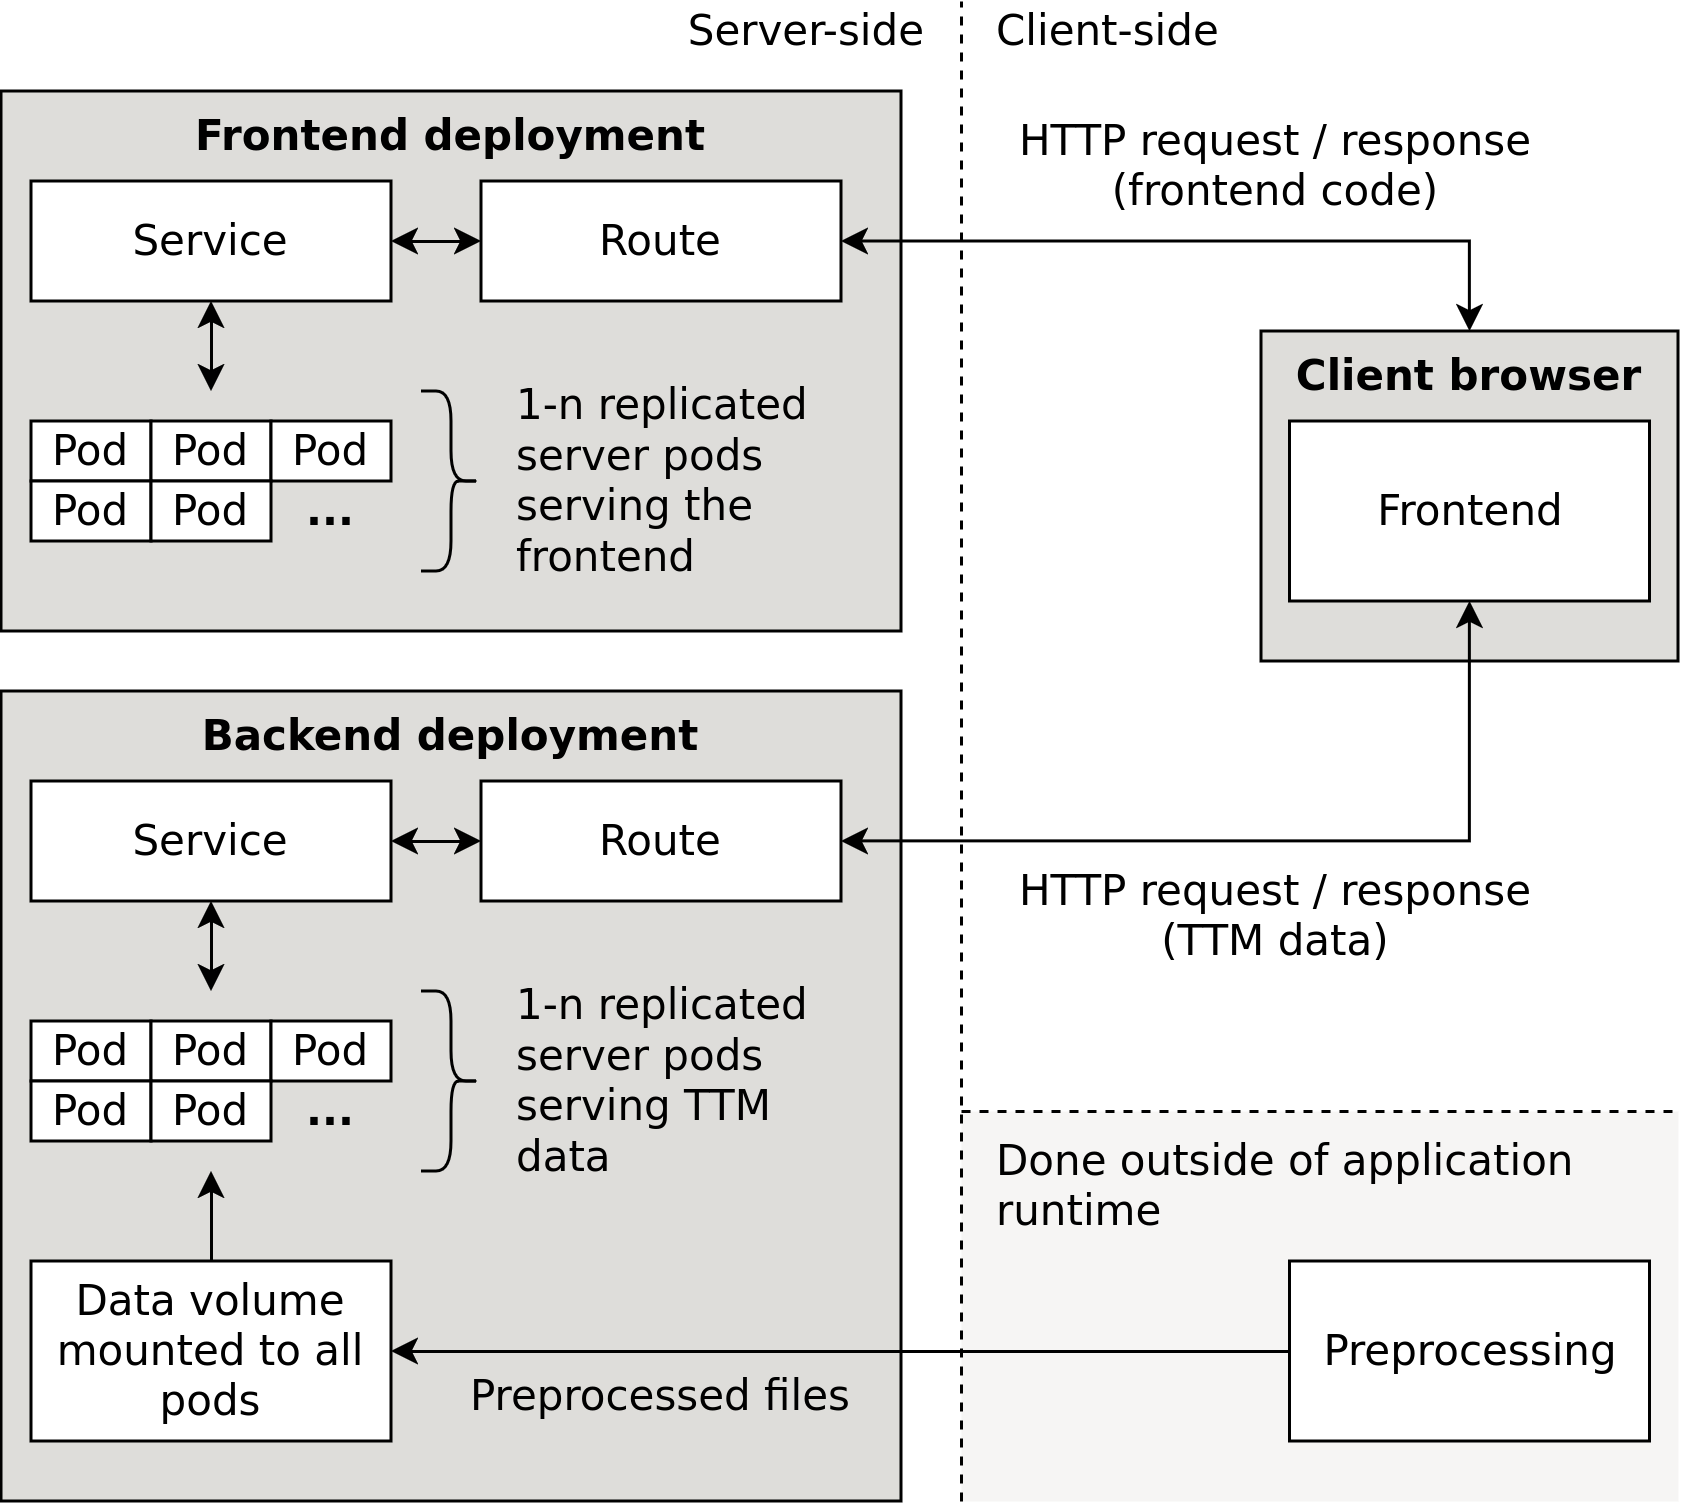
\includegraphics[width=\diagramwidth]{visual/figures/diagrams/architecture.png}
	\caption{Architecture}
	\label{fig:architechture}
\end{figure}

In short, containerization refers to a set of technologies
that enables packaging software and all its necessary components
into self-contained \textit{container images} that can be run as is,
regardless of the specifics of the underlying system.

SIDENOTE: I'll add figures of the components (at least the map application) here as suggested by Pyry.


% The need for serving (backend)
% - why data must be decoupled
% && the requirements serving must satisfy

% Different approaches

% Why nginx + static files?

% Describe how it was done

\subsection{Survey}

\subsubsection{Questionnaire design and structure}

The questionnaire is structured to:
\begin{itemize}
	\item Prompt the participant to use the map for different tasks
	\item Ask questions about the participant's experience
	on using the map for completing the tasks
\end{itemize}

Reasoning about the design: online questionnaire, tasks composed of prompts and questions.
Descriptions of what the purpose of each task was.

\subsubsection{Questionnaire distribution and participants}
How the survey was distributed,
Description of the sample.

(Response plots in appendices)
